\documentclass[aspectratio=169]{beamer}

% Default packages
\usepackage[T1]{fontenc}
\usepackage[english]{babel}
\usepackage{csquotes}
\usepackage{pgfplots}
\pgfplotsset{compat=newest}
\usepackage{booktabs}
\usepackage{siunitx}
\usepackage{amsmath}
\usepackage[backend=bibtex,style=authoryear]{biblatex}
\usepackage[ruled]{algorithm2e}
\bibliography{bibliography.bib}

% Removes icon in bibliography
\setbeamertemplate{bibliography item}{}

% Font selection
% Latin Modern
\usepackage{lmodern}
% Verdana font type
%\usepackage{verdana}
% Helvetica
%\usepackage{helvet}
% Times (text and math)
%\usepackage{newtx, newtxmath}
% Nice font combination
%\usepackage{mathptmx} % math
%\usepackage{sourcesanspro} % sans-serif
\usepackage{charter} % serif

%Avoid shaded in RMarkdown

% Use DTU theme, see below for options
\usetheme[department=compute]{DTU}

\title[Automated and Early Detection of Disease Outbreaks]{Automated and
Early Detection of Disease Outbreaks}
\author{\textbf{Kasper Schou Telkamp}\\
Supervisors: Jan Kloppenborg Møller, Lasse Engbo Christiansen}
\institute{\strut \\
\strut \\
Master Thesis Project\\
Spring, 2023\\
Technical University of Denmark}
\date{2023-09-20}
	
\newcommand{\tabitem}{{\color{dtured}$\bullet$} }

\DeclareMathOperator{\E}{E}
\DeclareMathOperator{\V}{V}
\DeclareMathOperator{\G}{G}
\DeclareMathOperator{\N}{N}
\DeclareMathOperator{\NB}{NB}
\DeclareMathOperator{\LN}{LN}
\DeclareMathOperator{\Pois}{Pois}
\DeclareMathOperator{\Geom}{Geom}

\setbeamercovered{transparent}

\begin{document}


\frame{
	\maketitle
}

\hypertarget{introduction}{%
\section{Introduction}\label{introduction}}

\hypertarget{about-me}{%
\subsection{About me}\label{about-me}}

\begin{frame}{About me}
\begin{columns}
\begin{column}{.48\textwidth}
\begin{itemize}
  \item MSc Eng., Quantitative Biology and Disease Modelling @ DTU
  \item Wife and three kids @ Vedbæk
  \item Passionate about e-Sports, particularly Counter Strike
\end{itemize}
\end{column}
\hfill
\begin{column}{.48\textwidth}

 \tiny


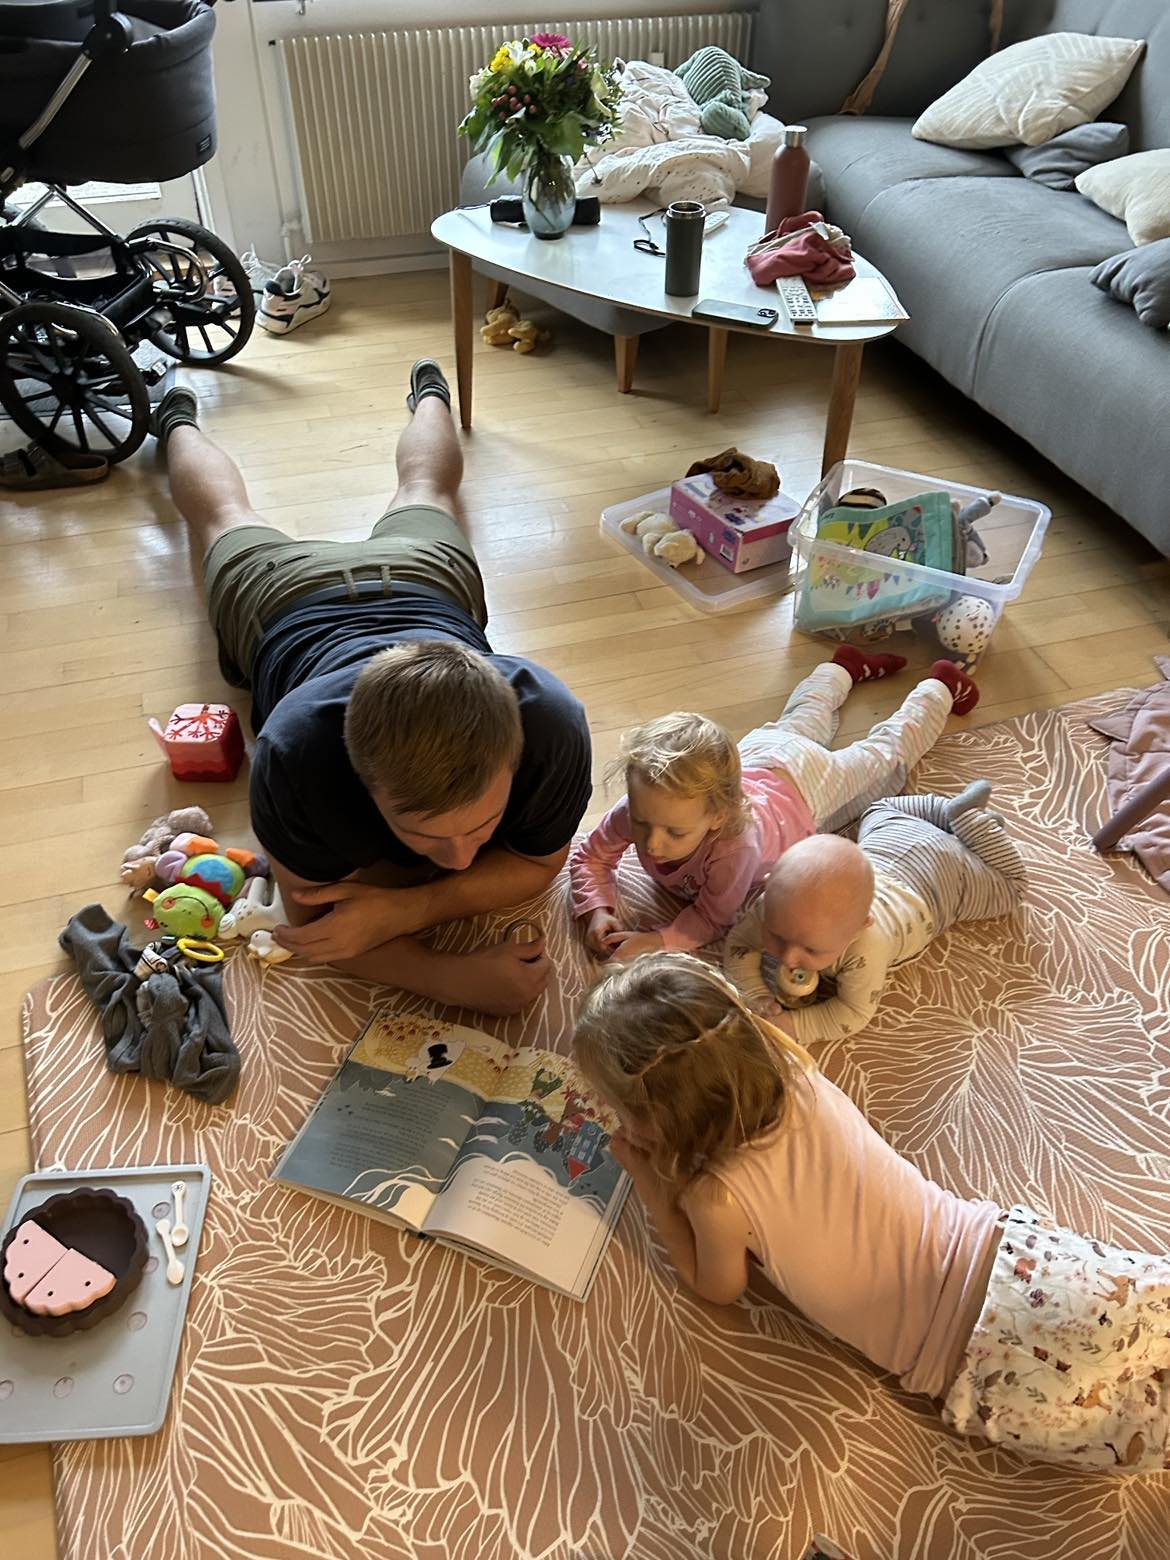
\includegraphics[width=0.75\linewidth]{../figures/family} 

 \normalsize
\end{column}
\end{columns}
\end{frame}

\hypertarget{about-disease-dynamics-forecasting-epidemiology-research}{%
\subsection{About Disease Dynamics \& Forecasting @ Epidemiology
Research}\label{about-disease-dynamics-forecasting-epidemiology-research}}

\begin{frame}{About Disease Dynamics \& Forecasting @ Epidemiology
Research}
\begin{columns}
\begin{column}{.68\textwidth}
\begin{itemize}
  \item Establish and maintain a model preparedness
  \begin{itemize}
    \item Improve understanding of immunity over time
    \item Manage lineages and mutations
  \end{itemize}
  \item Wastewater monitoring
  \item Signal detection - automatically identify potential outbreaks
  \item Analyze and model excess mortality
  \item Antimicrobial resistance
  \begin{itemize}
    \item Hospital network analysis - expansion of MiBAlert
    \item Focus on resistance in the population and its burden
  \end{itemize}
  \item One Health
\end{itemize}
\end{column}
\hfill
\begin{column}{.28\textwidth}

 \tiny


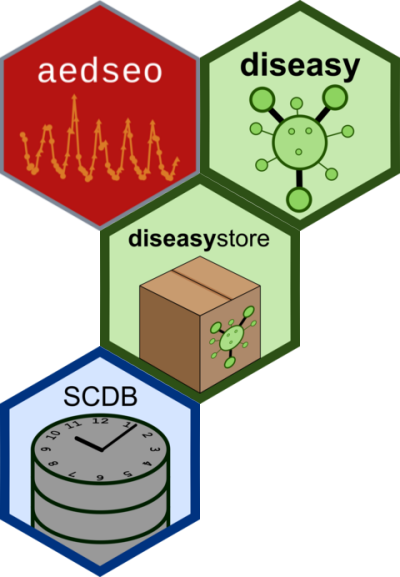
\includegraphics[width=0.75\linewidth]{../figures/r_packages} 

 \normalsize
\end{column}
\end{columns}
\end{frame}

\hypertarget{motivation}{%
\subsection{Motivation}\label{motivation}}

\begin{frame}{Motivation}
\begin{columns}
\begin{column}{.58\textwidth}
\begin{itemize}
  \item Establishment of MiBa by SSI in 2010
  \item Great opportunity for data analysis
  \item No fully automated procedures in place at SSI
\end{itemize}
\end{column}
\hfill
\begin{column}{.38\textwidth}

 \tiny



\includegraphics[width=0.75\linewidth]{../figures/MiBaPetriComp} 
\includegraphics[width=0.75\linewidth]{../figures/MiBa} 

 \normalsize
\end{column}
\end{columns}
\end{frame}

\hypertarget{algorithms-for-prospective-disease-outbreak-detection}{%
\section{Algorithms for prospective disease outbreak
detection}\label{algorithms-for-prospective-disease-outbreak-detection}}

\hypertarget{state-of-the-art-algorithms}{%
\subsection{State-of-the-art
algorithms}\label{state-of-the-art-algorithms}}

\begin{frame}{State-of-the-art algorithms}
State-of-the-art algorithms for aberration detection is presented in
\cite{Salmon_2016} and implemented in the R package
\textbf{surveillance}. The R package includes the method introduced by
\cite{Farrington_1996} together with the subsequently improved method
proposed by \cite{Noufaily_2013}.
\end{frame}

\hypertarget{novel-algorithm}{%
\subsection{Novel algorithm}\label{novel-algorithm}}

\begin{frame}{Novel algorithm}
The novel algorithm utilizes a generalized mixed effects model or a
hierarchical mixed effects model as a modeling framework to model the
count case observations \(\boldsymbol y\) and assess the unobserved
random effects \(\boldsymbol u\). These random effects are used directly
to characterize an outbreak.
\end{frame}

\begin{frame}{Formulation of hierarchical models}
\protect\hypertarget{formulation-of-hierarchical-models}{}
\only<1>{
\begin{align*}
  \mathbf{Pois}&\mathbf{son} \ \mathbf{Normal} & \mathbf{Pois}&\mathbf{son} \ \mathbf{Gamma} \\
  \boldsymbol{Y|u} &\sim \Pois \big( \boldsymbol{\lambda} \exp(\boldsymbol{u}) \big) & \boldsymbol{Y|u} &\sim \Pois (\boldsymbol{\lambda u}) \\
  \boldsymbol{u} &\sim \N(\boldsymbol{0},I\sigma^2) & \boldsymbol{u} &\sim \G(\boldsymbol 1/\phi,\phi)
\end{align*}
}
\only<2>{
\begin{align*}
  \mathbf{Pois}&\mathbf{son} \ \mathbf{Normal} & \mathbf{Pois}&\mathbf{son} \ \mathbf{Gamma} \\
  \boldsymbol{Y|u} &\sim \Pois \big( \boldsymbol{\lambda} \exp(\boldsymbol{u}) \big) & \boldsymbol{Y|u} &\sim \Pois (\boldsymbol{\lambda u}) \\
  \boldsymbol{u} &\sim \N(\boldsymbol{0},I\sigma^2) & \boldsymbol{u} &\sim \G(\boldsymbol 1/\phi,\phi) \\
  & & & \\
  & & Y&\sim\NB\big(1/\phi,1/(\lambda\phi+1)\big)
\end{align*}
}
\end{frame}

\begin{frame}{Step 1: Modeling framework}
\protect\hypertarget{step-1-modeling-framework}{}
\begin{itemize}
  \item Assume a hierarchical Poisson Normal or Poisson Gamma model to reference data using a log link
  \item Incorporate covariates by supplying a model formula on the form
  \begin{equation}
    \log(\lambda_{it})=\boldsymbol x_{it}\boldsymbol \beta+\log(n_{it}), \quad i=1,\dots,m, \quad t=1,\dots,T
  \end{equation}
  \item Account for structural changes in the time series using a rolling window of width $k$
\end{itemize}
\end{frame}

\begin{frame}{Step 2: Inference of random effects}
\protect\hypertarget{step-2-inference-of-random-effects}{}
\begin{itemize}
  \item Infer one-step ahead random effects $\hat u_{i{t_1}}$ for each group using the fitted model
  \item Define outbreak detection threshold $U_{t_0}$ as a quantile of the second stage model's random effects distribution
  \item Use either a Gaussian or Gamma distribution with respective plug-in estimates
\end{itemize}
\end{frame}

\begin{frame}{Step 3: Parameter estimations and outbreak detection}
\protect\hypertarget{step-3-parameter-estimations-and-outbreak-detection}{}
\begin{itemize}
  \item Compare inferred random effects $\hat u_{i{t_1}}$ to a threshold $U_{t_0}$
  \item Raise and alarm if the inferred random effect exceeds the threshold, i.e. $\hat u_{i{t_1}}>U_{t_0}$
  \item Omit outbreak related observations from future parameter estimation
\end{itemize}
\end{frame}

\hypertarget{case-study}{%
\section{Case study}\label{case-study}}

\hypertarget{shiga-toxin-verotoxin-producing-escherichia-coli-stec}{%
\subsection{\texorpdfstring{Shiga toxin (verotoxin)-producing
\emph{Escherichia coli}
(STEC)}{Shiga toxin (verotoxin)-producing Escherichia coli (STEC)}}\label{shiga-toxin-verotoxin-producing-escherichia-coli-stec}}

\begin{frame}{Shiga toxin (verotoxin)-producing \emph{Escherichia coli}
(STEC)}
\tiny

\begin{figure}[H]
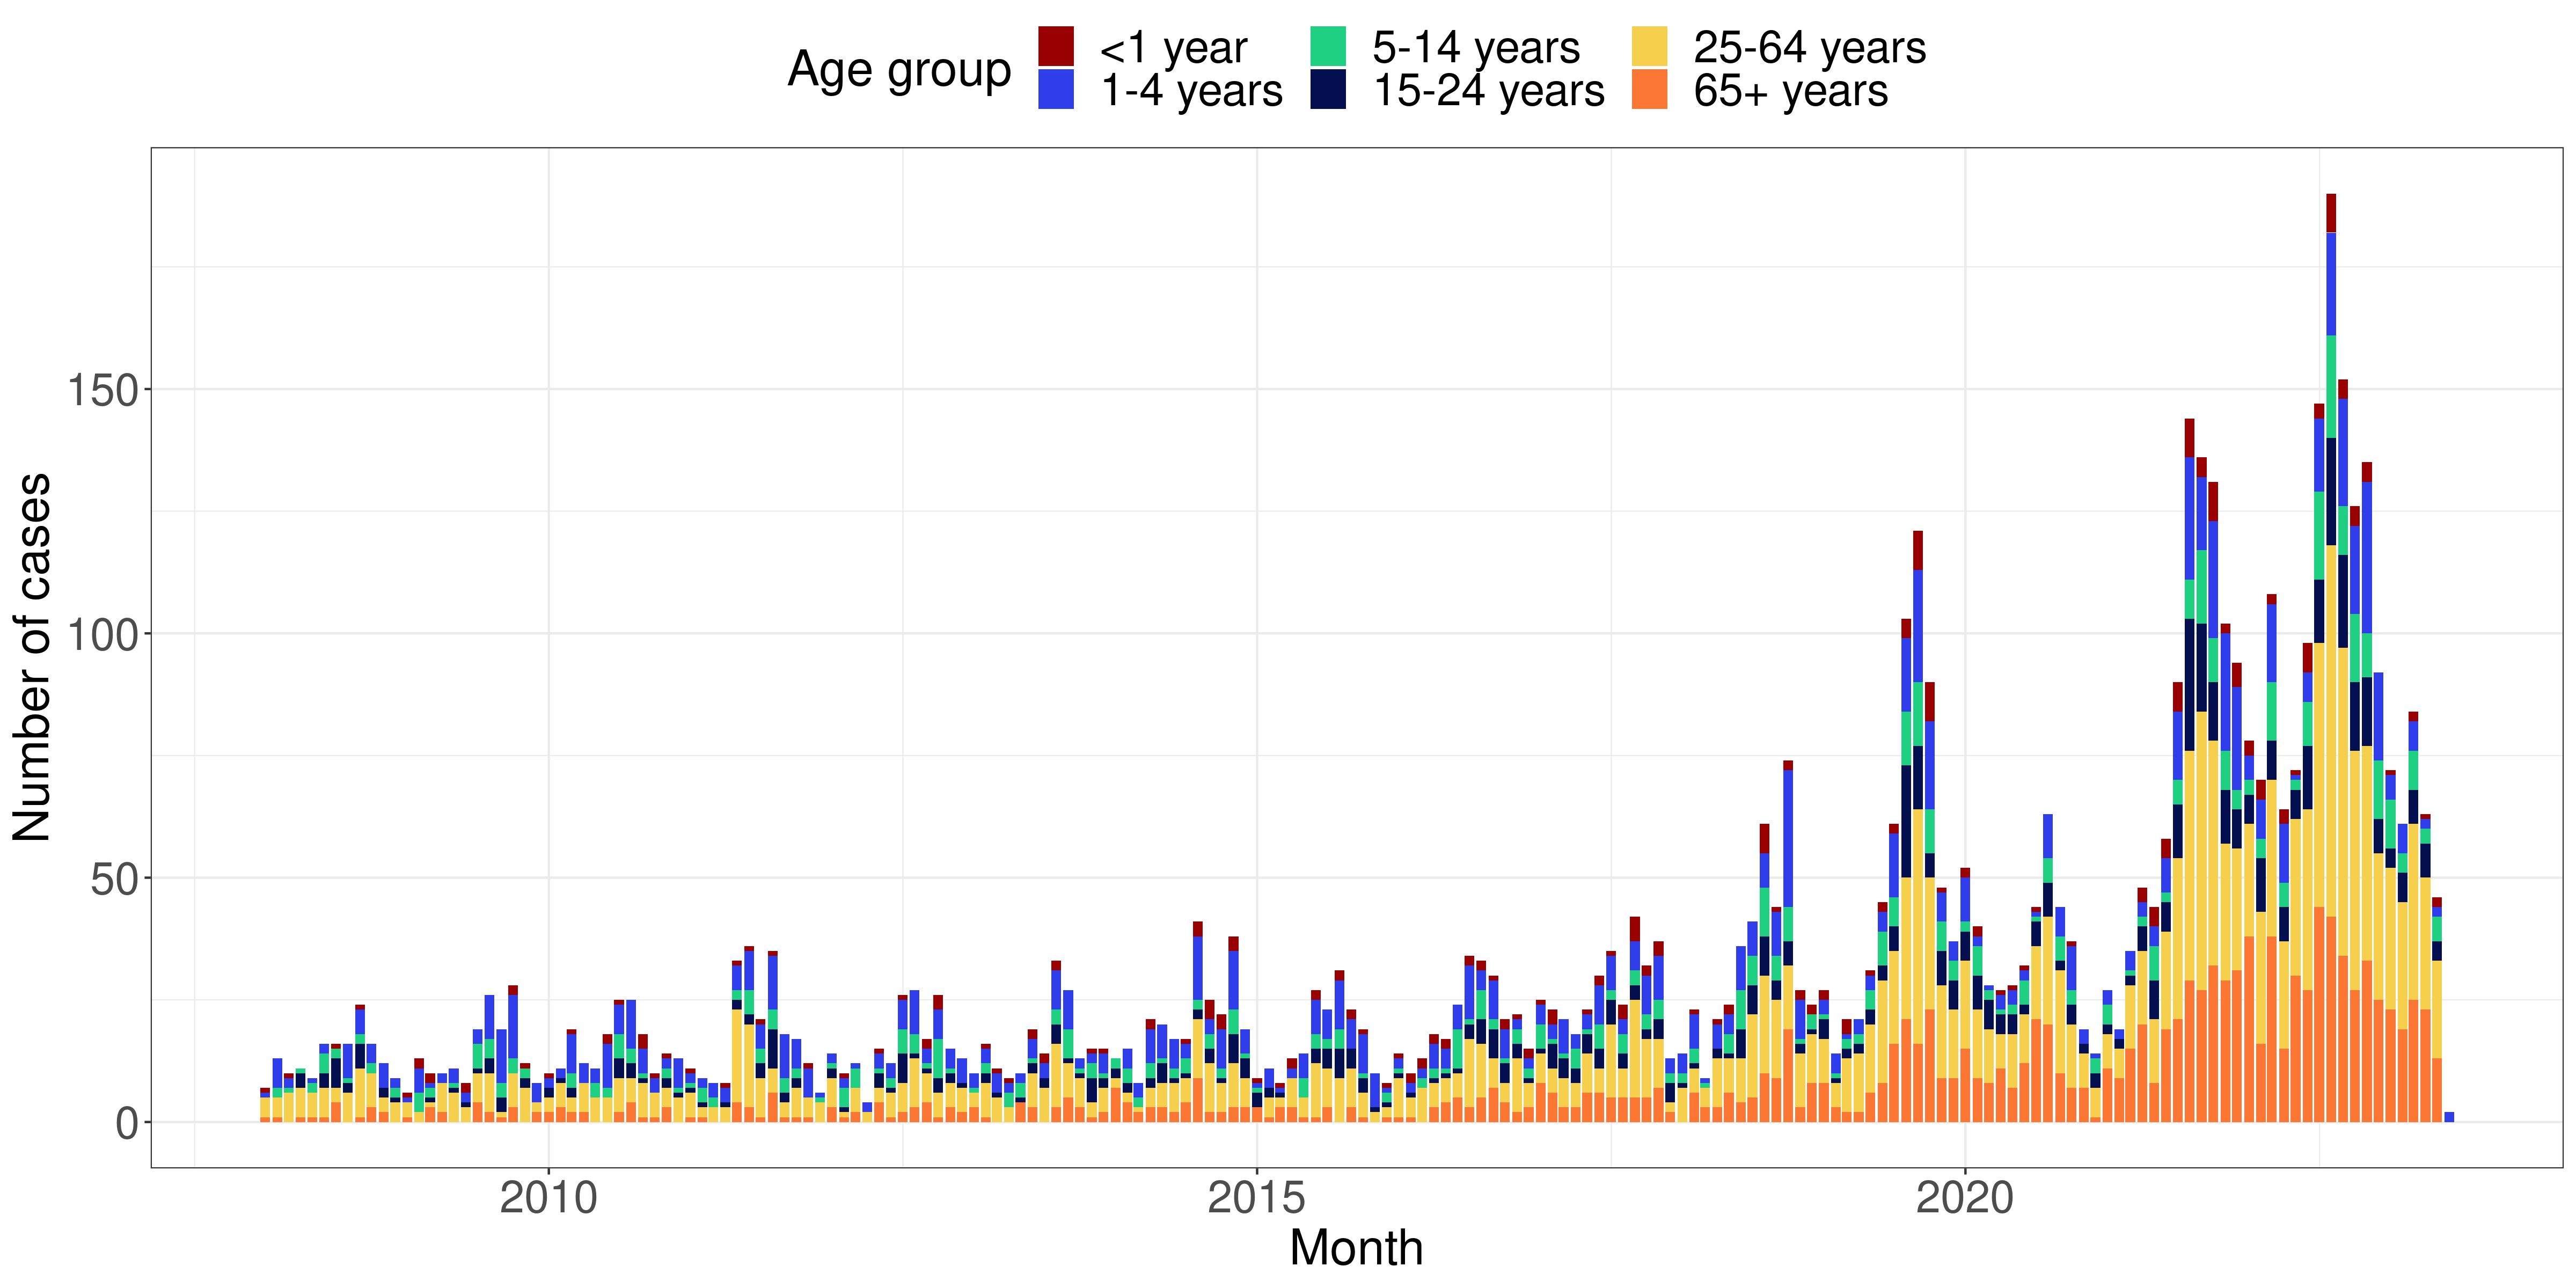
\includegraphics[width=0.75\linewidth]{../figures/STEC_long_plot} \caption{A stacked bar graph illustrating the number of monthly STEC cases observed in the period from 2008 to 2022 for the six age groups.}\label{fig:STEC}
\end{figure}

\normalsize
\end{frame}

\hypertarget{constant-model}{%
\subsection{Constant model}\label{constant-model}}

\begin{frame}{Constant model}
\begin{equation}\label{eq:Agegroup}
  \log(\lambda_{it}) = \beta(ageGroup_{i}) + \log(n_{it})
\end{equation}

\begin{itemize}
  \item $\lambda_{it}$ is the outbreak intensity at time $t$ for age group $i$
  \item $\beta(ageGroup_{i})$ is the fixed effect specific to age group $i$
  \item $\log(n_{it})$ acts as an offset, accounting for the population size at time $t$ for age group $i$
\end{itemize}
\end{frame}

\hypertarget{trend-model}{%
\subsection{Trend model}\label{trend-model}}

\begin{frame}{Trend model}
\begin{equation}
  \log(\lambda_{it})=\beta(ageGroup_{i}) + \beta_{trend} t + \log(n_{it})
\end{equation}

\begin{itemize}
  \item In addition to constant model, includes a trend component
  \item $\beta_{trend}$ quantifies the rate of change in the outbreak intensity over time
\end{itemize}
\end{frame}

\hypertarget{seasonality-model}{%
\subsection{Seasonality model}\label{seasonality-model}}

\begin{frame}{Seasonality model}
\begin{equation}
\log(\lambda_{it})=\beta(ageGroup_{i})+ \sin \bigg(\frac{2\pi\cdot \tau_t}{12}\bigg) \beta_{\sin} + \cos \bigg(2\frac{\pi\cdot \tau_t}{12}\bigg) \beta_{\cos} + \log(n_{it})
\end{equation}

\begin{itemize}
  \item In addition to constant model, incorporates an annual seasonality pattern
  \item $\tau_t$ represents the time period $t$ within a year (1-12)
  \item $\beta_{\sin}$ and $\beta_{\cos}$ capture the effect of the seasonal pattern
\end{itemize}
\end{frame}

\hypertarget{combined-trend-and-seasonality-model}{%
\subsection{Combined trend and seasonality
model}\label{combined-trend-and-seasonality-model}}

\begin{frame}{Combined trend and seasonality model}
\begin{equation}\label{eq:AgegroupTrendSeasonality}
  \log(\lambda_{it})=\beta(ageGroup_{i}) + \beta_{trend} t + \sin \bigg(\frac{2\pi\cdot \tau_t}{12}\bigg) \beta_{\sin} + \cos \bigg(\frac{2\pi\cdot \tau_t}{12}\bigg)\beta_{\cos} + \log(n_{it})
\end{equation}

\begin{itemize}
  \item Builds upon previous models, combining trend and seasonality components
  \item Includes both $\beta_{trend}$, $\beta_{\sin}$, and $\beta_{\cos}$ parameters
\end{itemize}
\end{frame}

\hypertarget{estimated-one-step-ahead-random-effects}{%
\subsection{Estimated one-step ahead random
effects}\label{estimated-one-step-ahead-random-effects}}

\begin{frame}{Estimated one-step ahead random effects}
\begin{columns}
\begin{column}{.50\textwidth}
\begin{itemize}
  \item<1> A rolling window of width $k=36$ months is employed
  \item<1> The combined model minimizes the logarithmic score  
  \item<1> Upper bound $U_{t_0}$ is based on the $90\%$ quantile of the random effects distribution
  \item<1> If the one-step ahead random effects $u_{it_1}$ exceeds $U_{t_0}$ an alarm is raised
\end{itemize}
\vspace{.1cm}
\begin{itemize}
  \item<2> 30 alarms are generated using the Poisson Normal framework, while 31 alarms are generated using the Poisson Gamma framework.
  \item<2> A great number of alarms are generated in the period from March 2021 to March 2022
\end{itemize}
\end{column}
\hfill
\begin{column}{.46\textwidth}

 \tiny


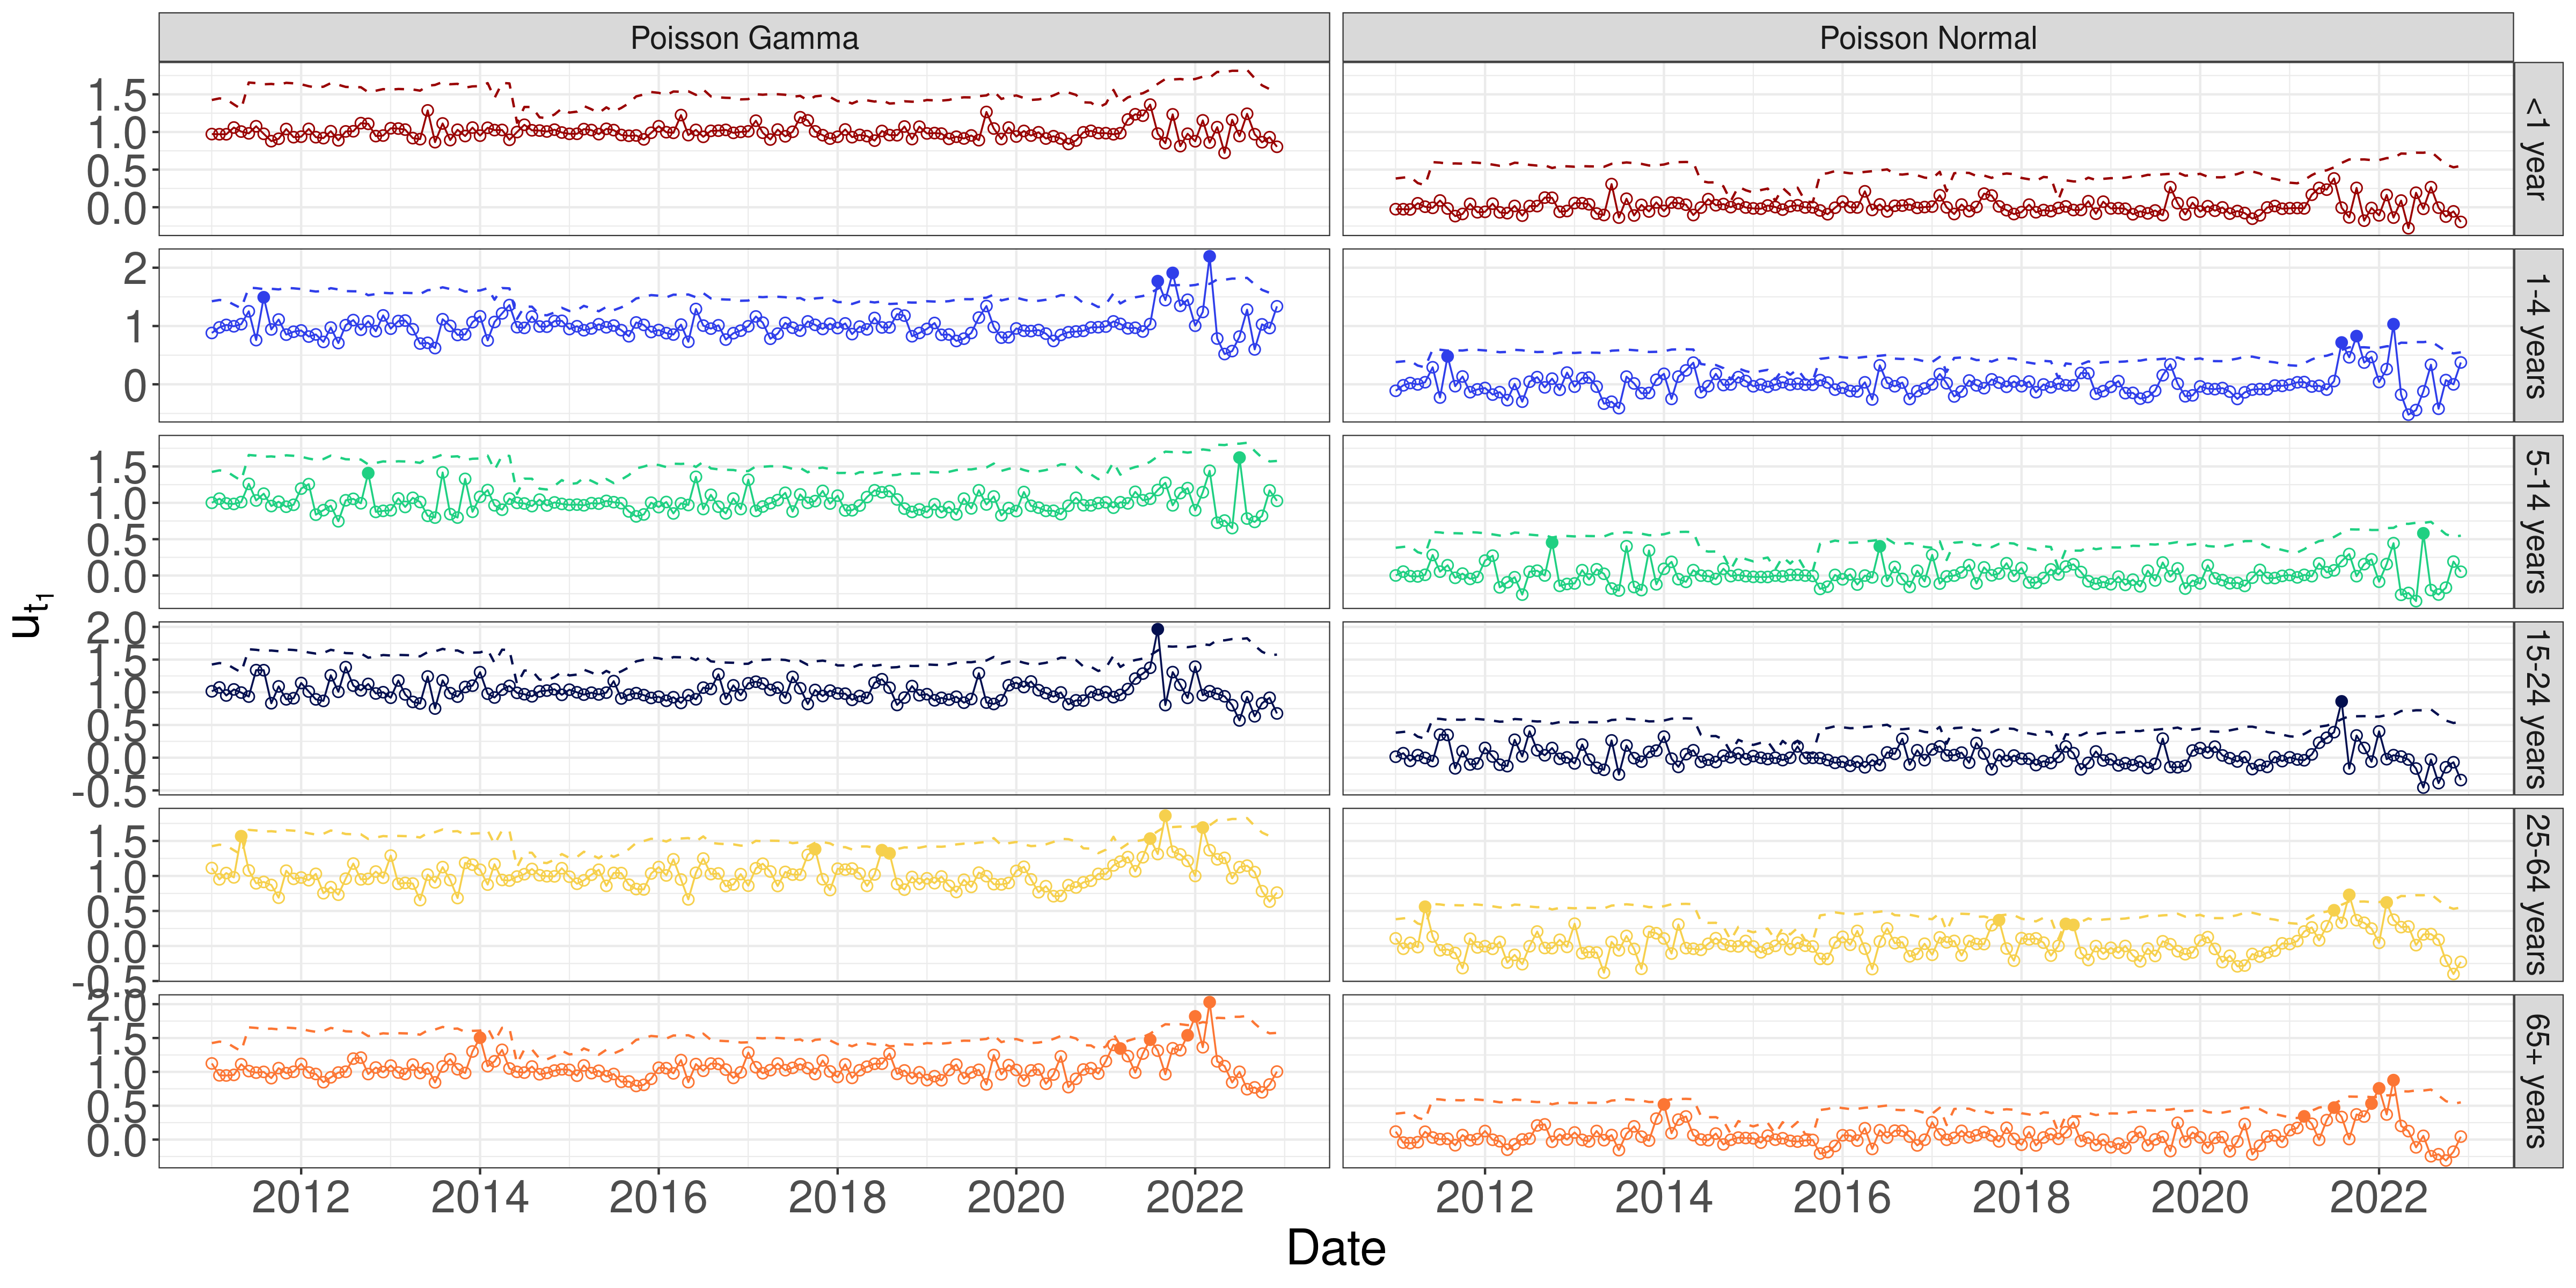
\includegraphics[width=1\linewidth]{../figures/Compare_novel_STEC} 

 \normalsize
\end{column}
\end{columns}
\end{frame}

\hypertarget{performance-of-statistical-outbreak-detection-algorithms}{%
\subsection{Performance of statistical outbreak detection
algorithms}\label{performance-of-statistical-outbreak-detection-algorithms}}

\begin{frame}{Performance of statistical outbreak detection algorithms}
\tiny

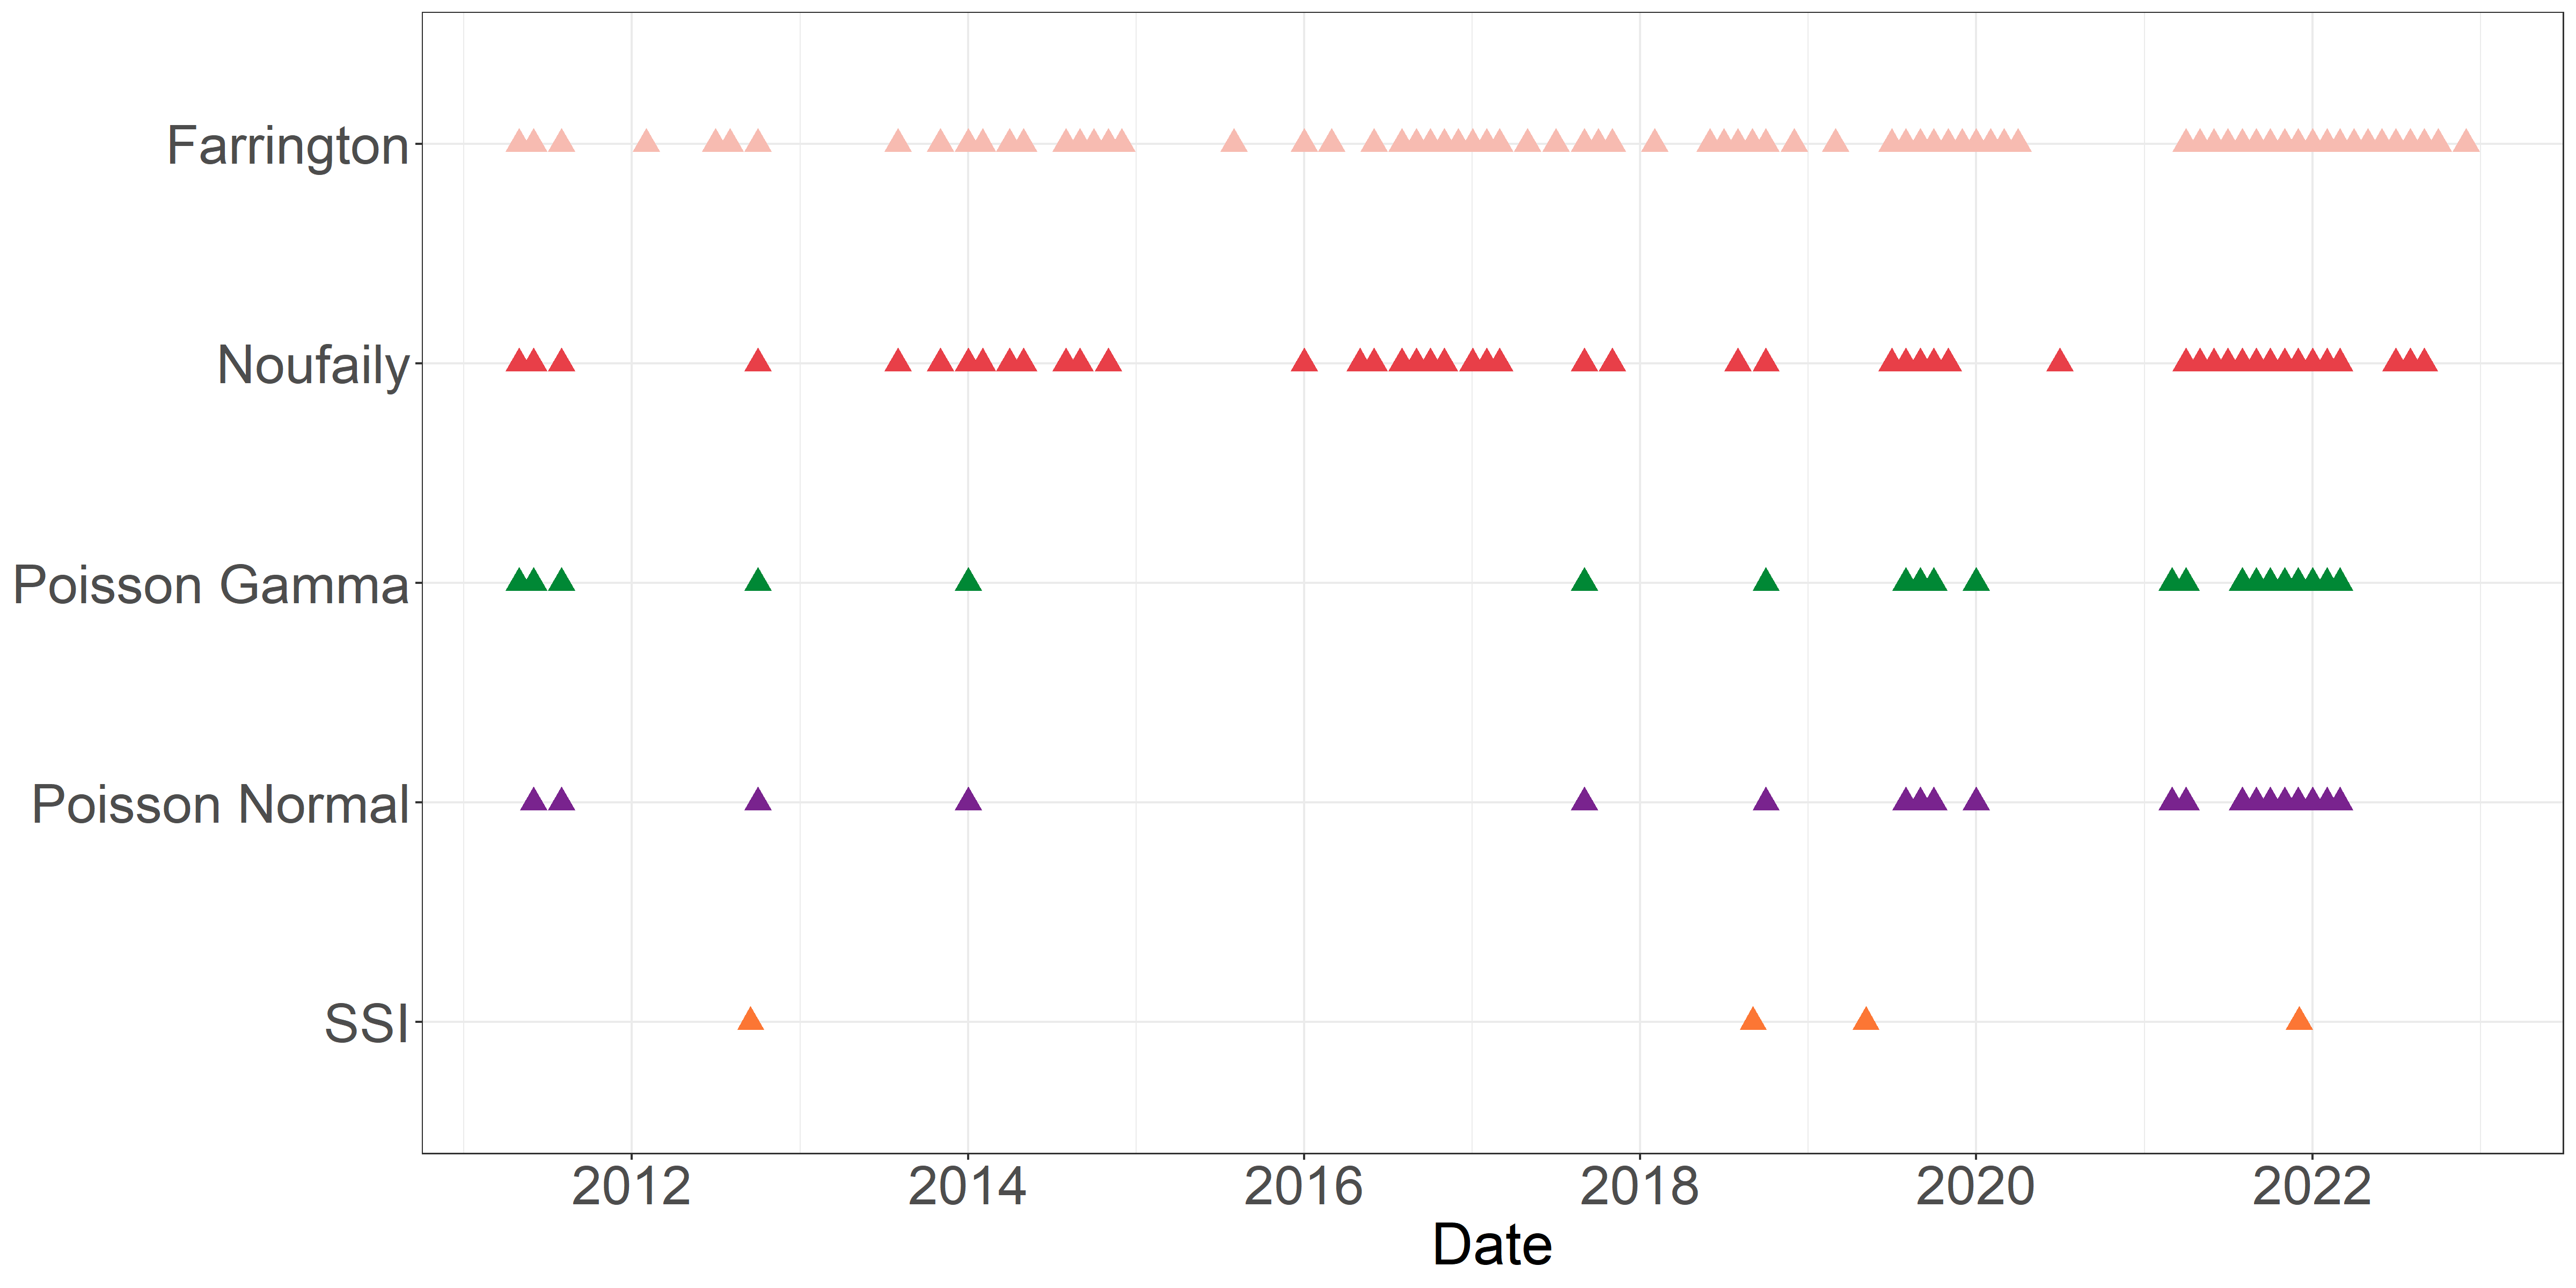
\includegraphics[width=1\linewidth]{../figures/Compare_alarms_STEC}

\normalsize
\end{frame}

\hypertarget{simulation-study}{%
\section{Simulation study}\label{simulation-study}}

\hypertarget{baseline-data}{%
\subsection{Baseline data}\label{baseline-data}}

\begin{frame}{Baseline data}
Simulated baseline data is generated according to a Negative Binomial
distribution with mean \(\mu\) and a variance parameter \(\phi\mu\). The
equation for the mean \(\mu(t)\) is given as:

\begin{equation}
\mu(t)=\exp\Biggl(\theta+\beta_{trend} t+\sum_{j=1}^m \biggl(\gamma_1 \cos\Bigl(\frac{2\pi jt}{52}\Bigl) + \gamma_2 \sin \Bigl(\frac{2\pi jt}{52} \Bigl)\biggl)\Biggl)
\end{equation}
\end{frame}

\hypertarget{scenarios}{%
\subsection{Scenarios}\label{scenarios}}

\begin{frame}{Scenarios}
\tiny

\begin{table}[H]
\centering\begingroup\fontsize{10}{12}\selectfont

\begin{tabular}[t]{llllllll}
\toprule
Scenario & $\theta$ & $\phi$ & $\beta$ & $\gamma_1$ & $\gamma_2$ & $m$ & Trend\\
\midrule
1 & 0.1 & 1.5 & 0.0000 & 0.00 & 0.00 & 0 & 0\\
2 & 0.1 & 1.5 & 0.0000 & 0.60 & 0.60 & 1 & 0\\
3 & 0.1 & 1.5 & 0.0025 & 0.00 & 0.00 & 0 & 1\\
4 & 0.1 & 1.5 & 0.0025 & 0.60 & 0.60 & 1 & 1\\
\addlinespace
5 & -2.0 & 2.0 & 0.0000 & 0.00 & 0.00 & 0 & 0\\
6 & -2.0 & 2.0 & 0.0000 & 0.10 & 0.30 & 1 & 0\\
7 & -2.0 & 2.0 & 0.0050 & 0.00 & 0.00 & 0 & 1\\
8 & -2.0 & 2.0 & 0.0050 & 0.10 & 0.30 & 1 & 1\\
\addlinespace
... & ... & ... & ... & ... & ... & ... & ...\\
\addlinespace
25 & 5.0 & 1.2 & 0.0000 & 0.00 & 0.00 & 0 & 0\\
26 & 5.0 & 1.2 & 0.0000 & 0.05 & 0.01 & 1 & 0\\
27 & 5.0 & 1.2 & 0.0001 & 0.00 & 0.00 & 0 & 1\\
28 & 5.0 & 1.2 & 0.0001 & 0.05 & 0.01 & 1 & 1\\
\bottomrule
\end{tabular}
\endgroup{}
\end{table}

\normalsize
\end{frame}

\hypertarget{scenarios-illustration}{%
\subsection{Scenarios illustration}\label{scenarios-illustration}}

\begin{frame}{Scenarios illustration}
\tiny

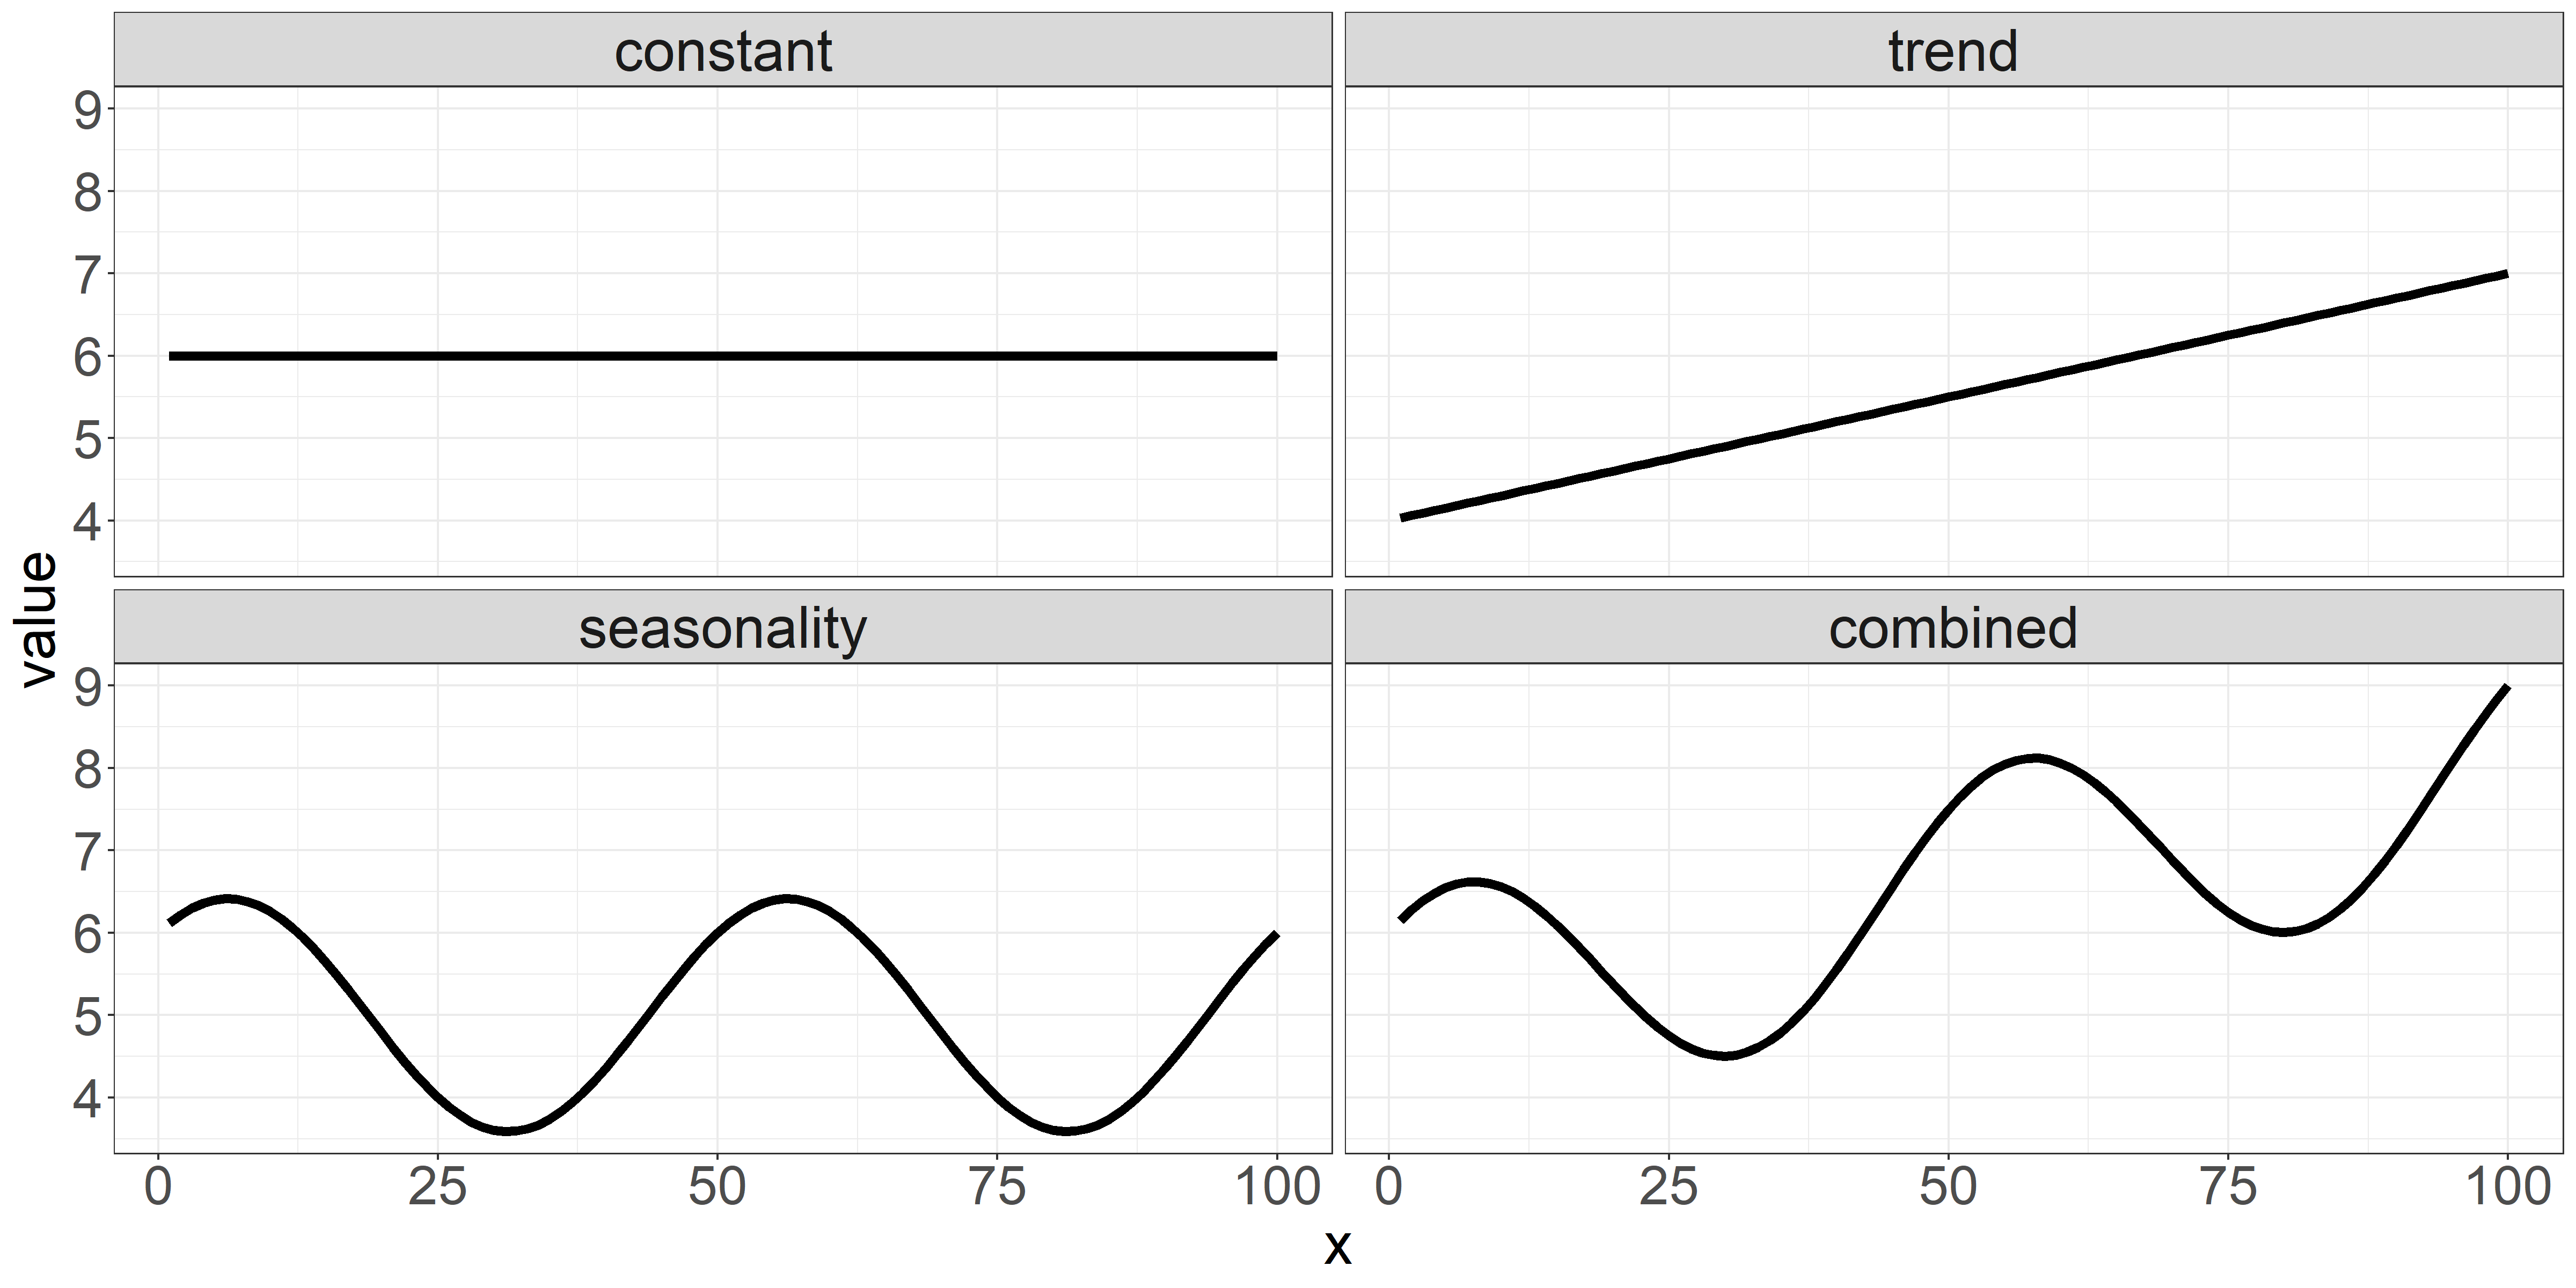
\includegraphics[width=1\linewidth]{../figures/scenarioIllustration}

\normalsize
\end{frame}

\hypertarget{outbreaks}{%
\subsection{Outbreaks}\label{outbreaks}}

\begin{frame}{Outbreaks}
\begin{columns}
\begin{column}{.50\textwidth}
\begin{itemize}
  \item Four outbreaks during baseline weeks (313-575), one outbreak during current weeks (576-624)
  \item Random constant value $k$ is chosen
  \item Outbreak size $v$ is generated from a Poisson distribution with mean equal to $k$ times the standard deviation from the baseline data
  \item The $v$ outbreak cases are distributed randomly in time according to a discretized log-normal distribution represented as $Z \sim \lfloor \LN(0,0.5^2)\rfloor$
\end{itemize}
\end{column}
\hfill
\begin{column}{.46\textwidth}

 \tiny

\begin{figure}[H]
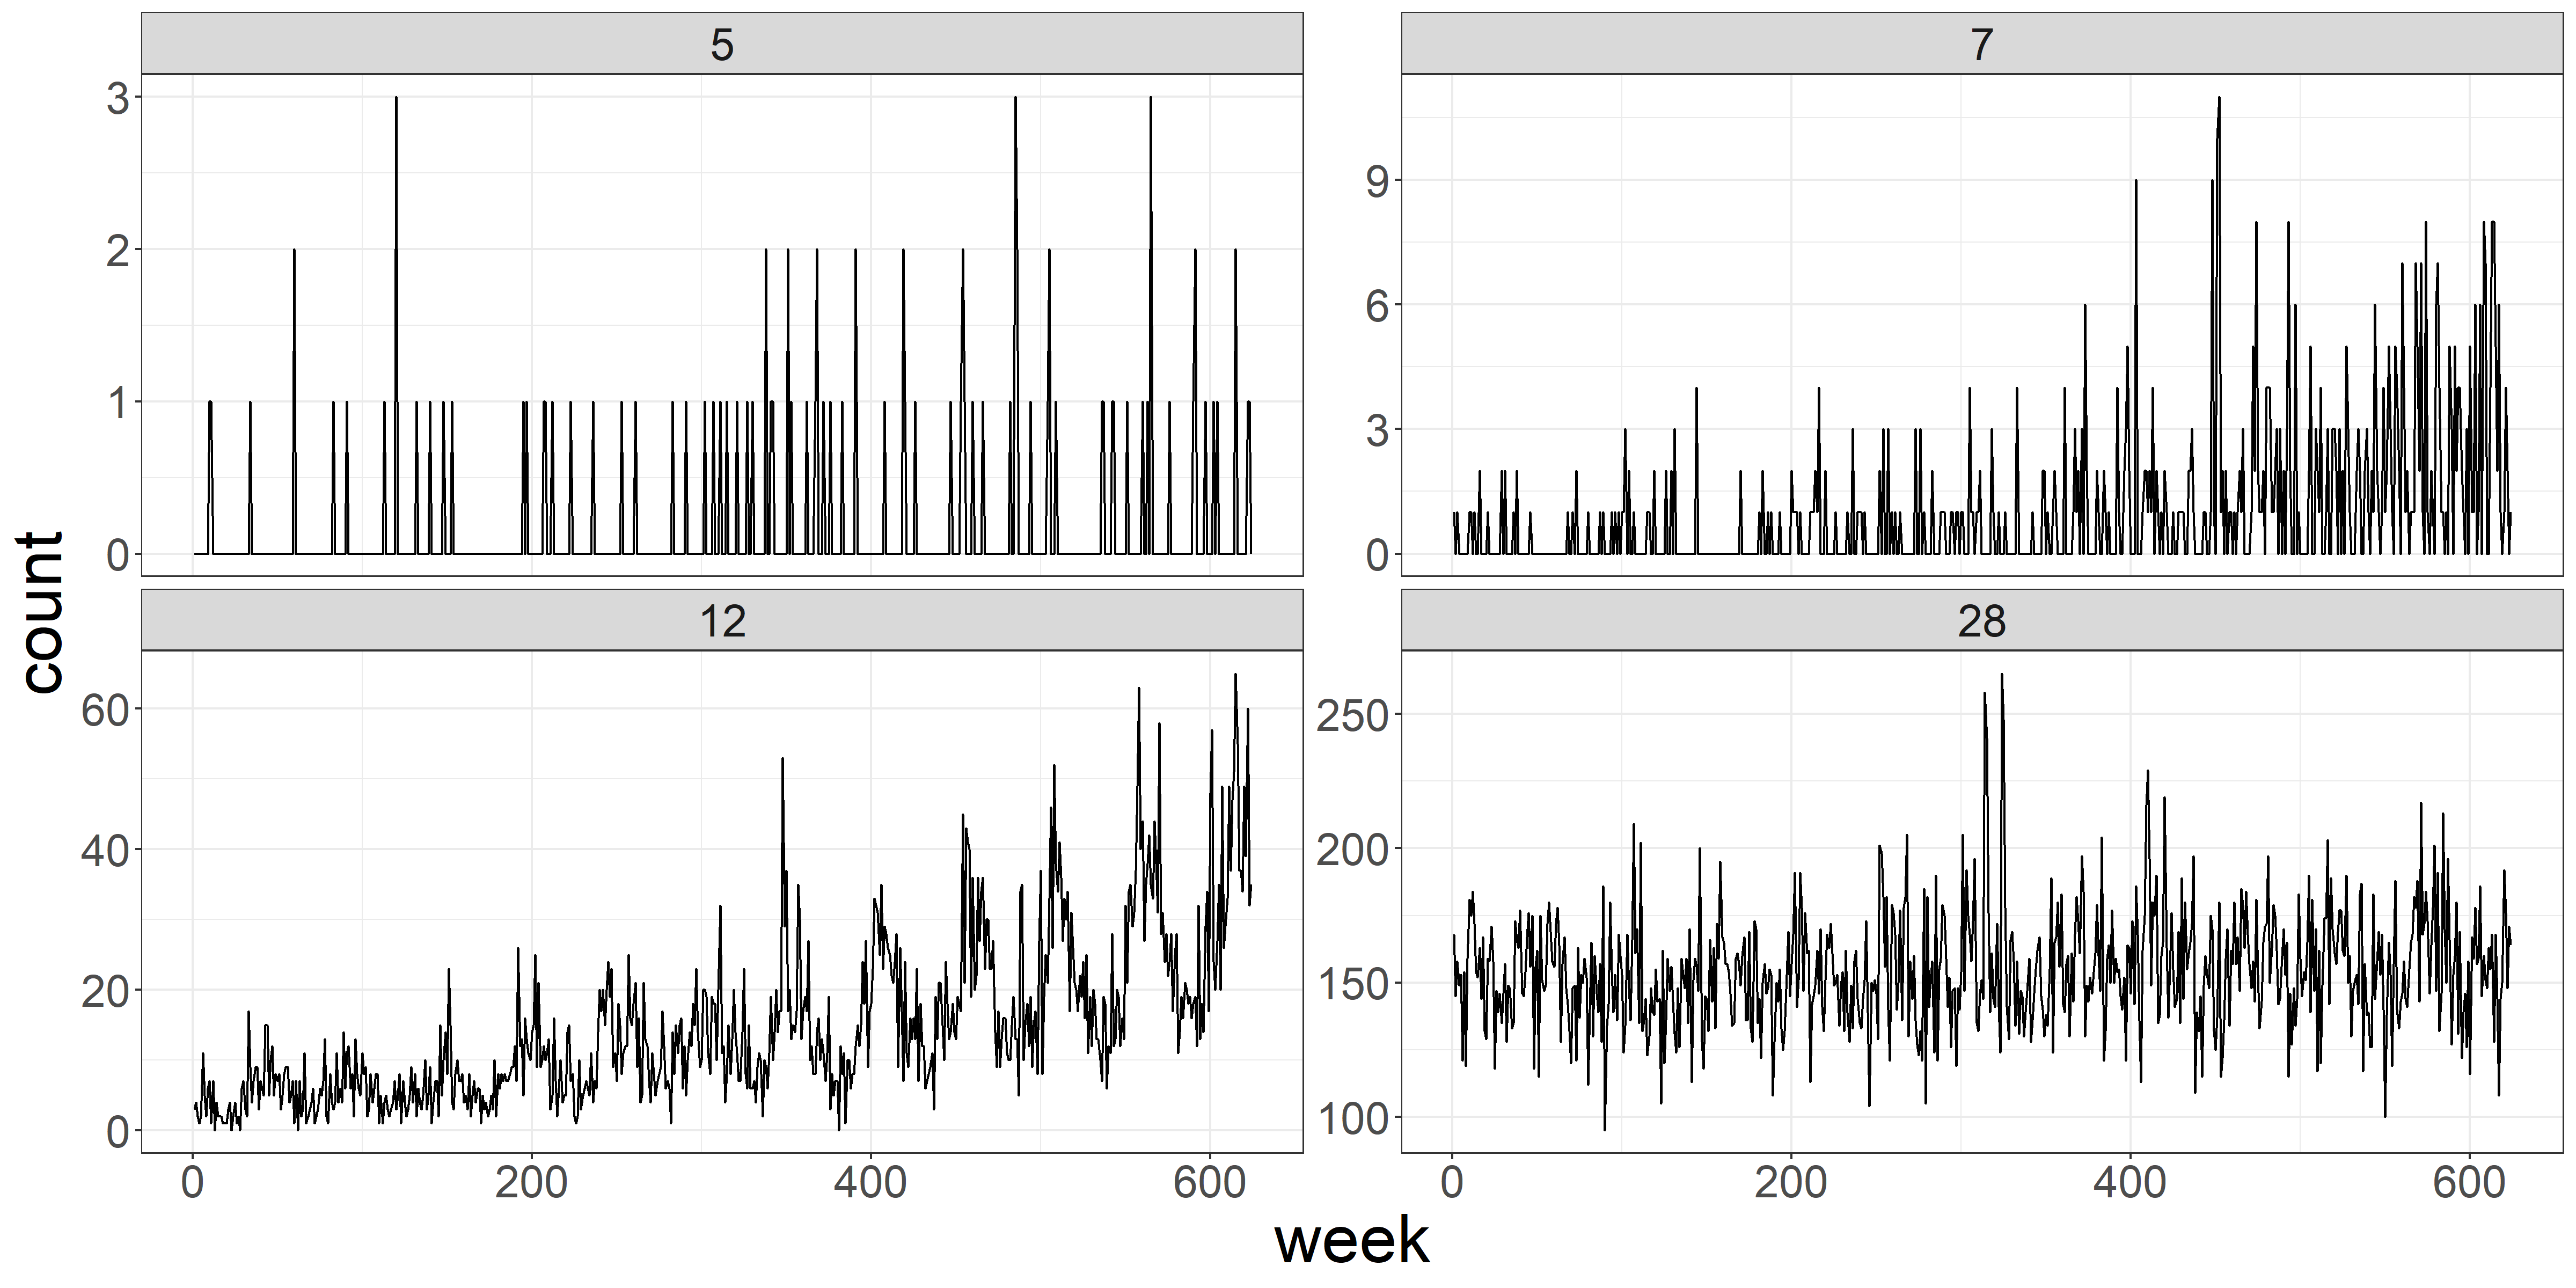
\includegraphics[width=1\linewidth]{../figures/Realizations} \caption{Plots of one randomly chosen realization for scenario 8, 12, 13, and 20.}\label{fig:Realizations}
\end{figure}

 \normalsize
\end{column}
\end{columns}
\end{frame}

\hypertarget{false-positive-rates}{%
\subsection{False Positive Rates}\label{false-positive-rates}}

\begin{frame}{False Positive Rates}
\tiny

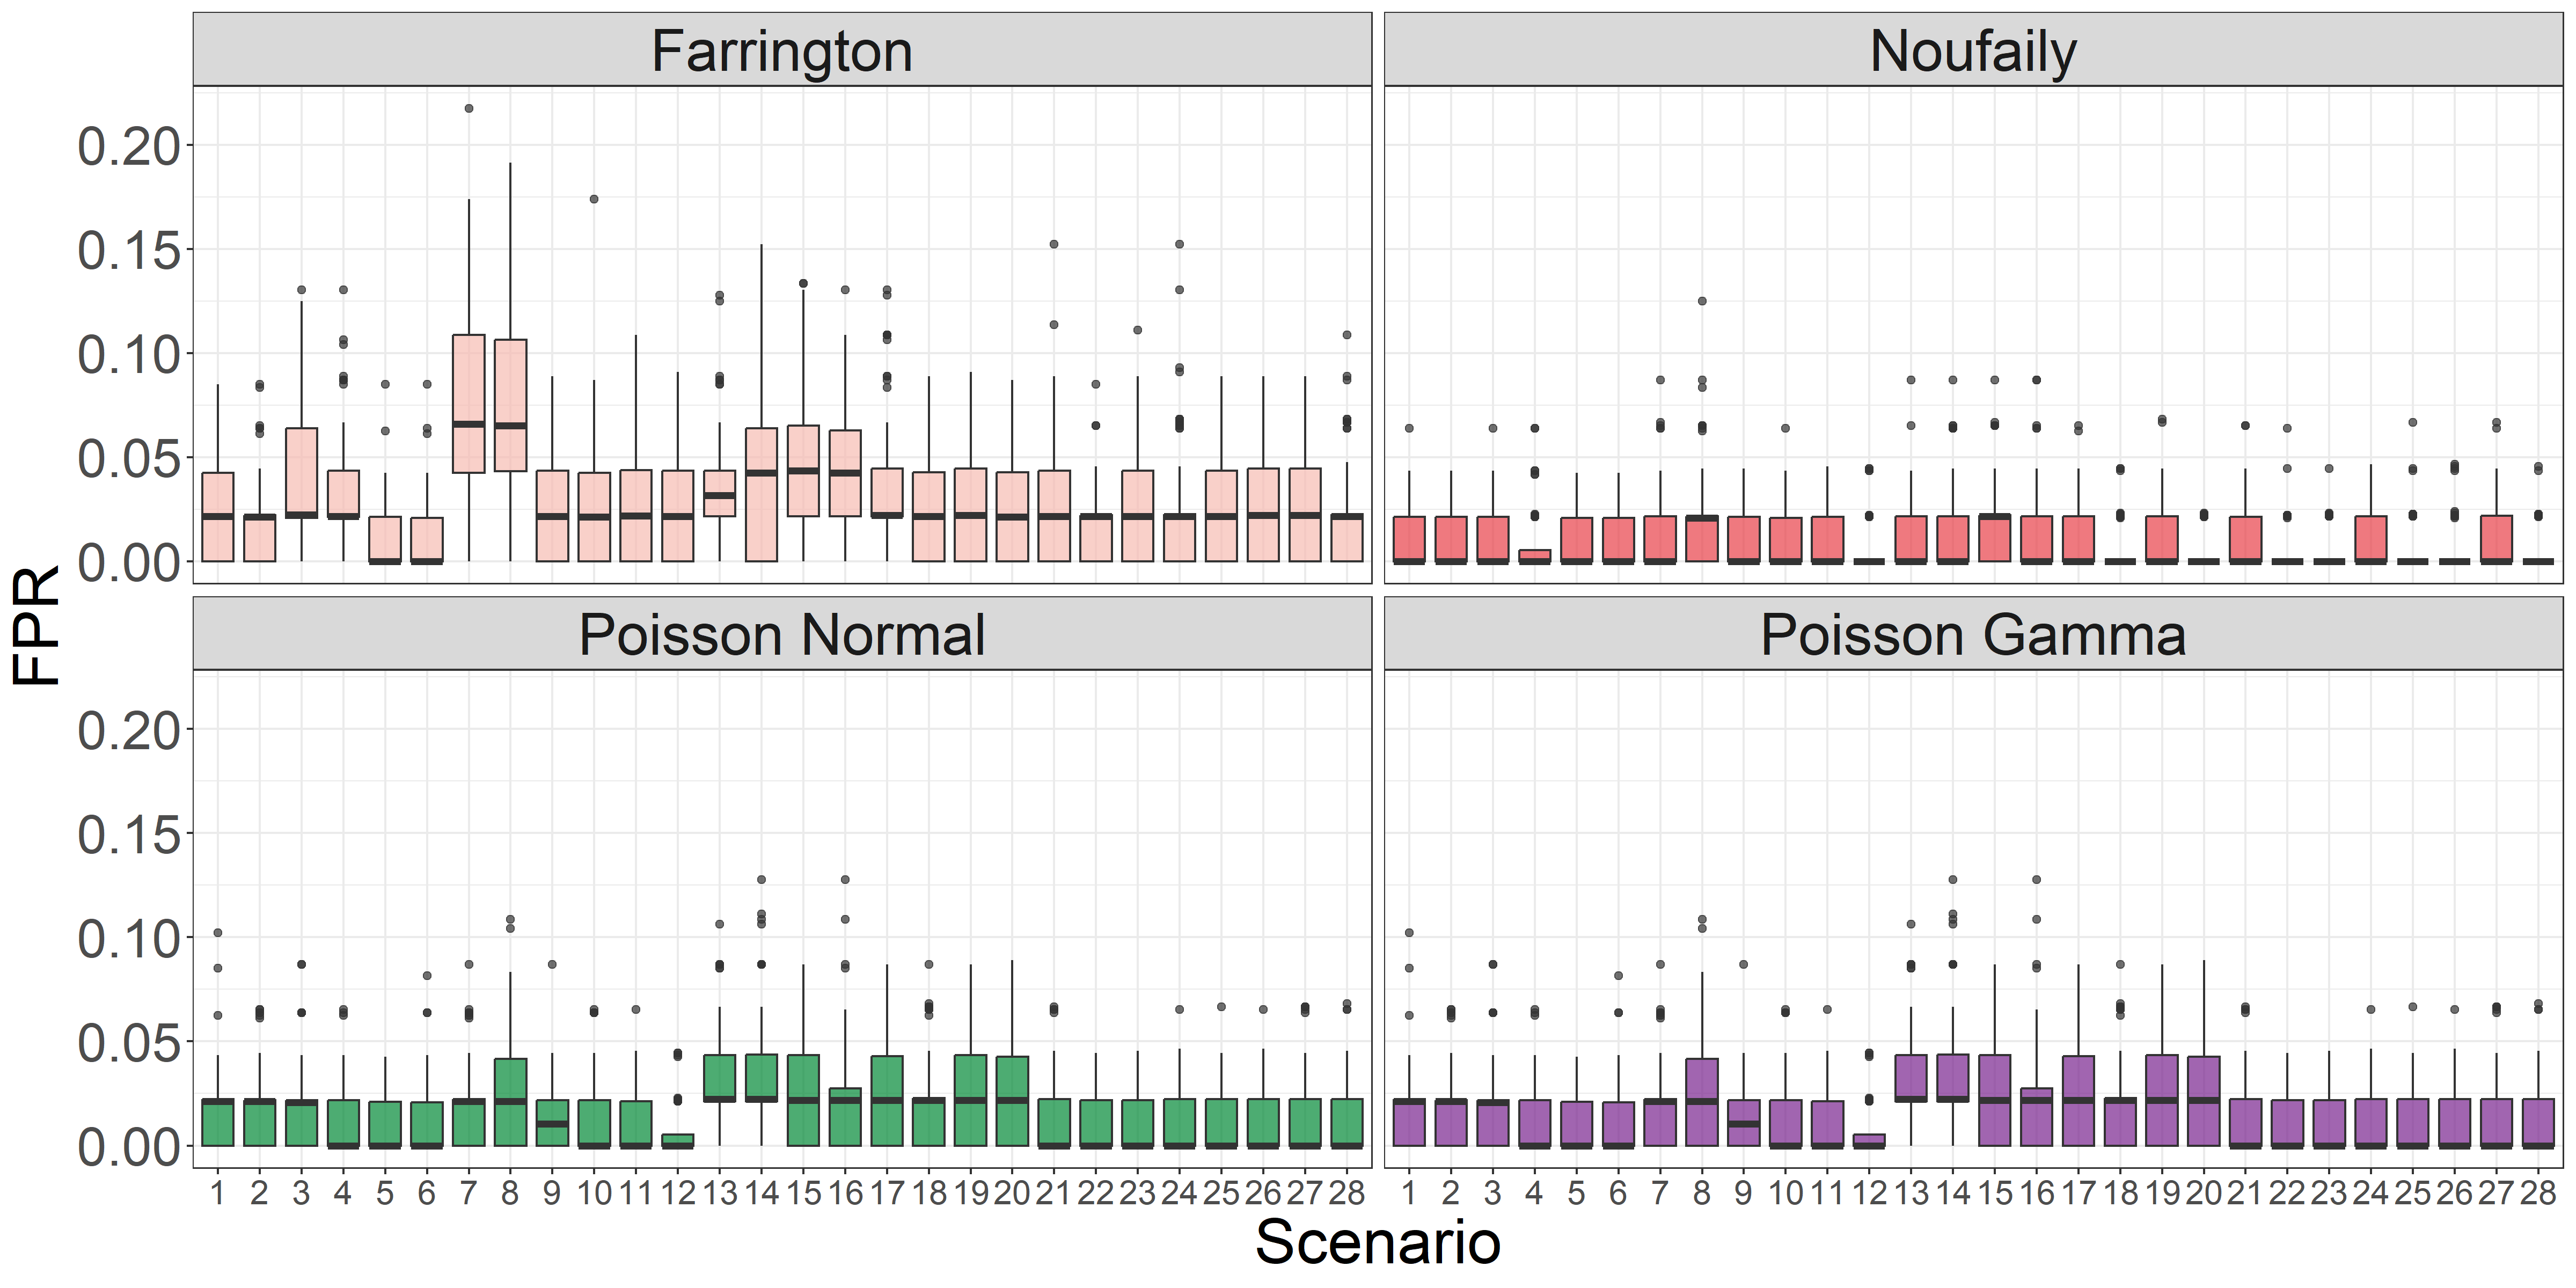
\includegraphics[width=1\linewidth]{../figures/FPRPlot}

\normalsize
\end{frame}

\hypertarget{probability-an-outbreak-is-detected}{%
\subsection{Probability an outbreak is
detected}\label{probability-an-outbreak-is-detected}}

\begin{frame}{Probability an outbreak is detected}
\tiny

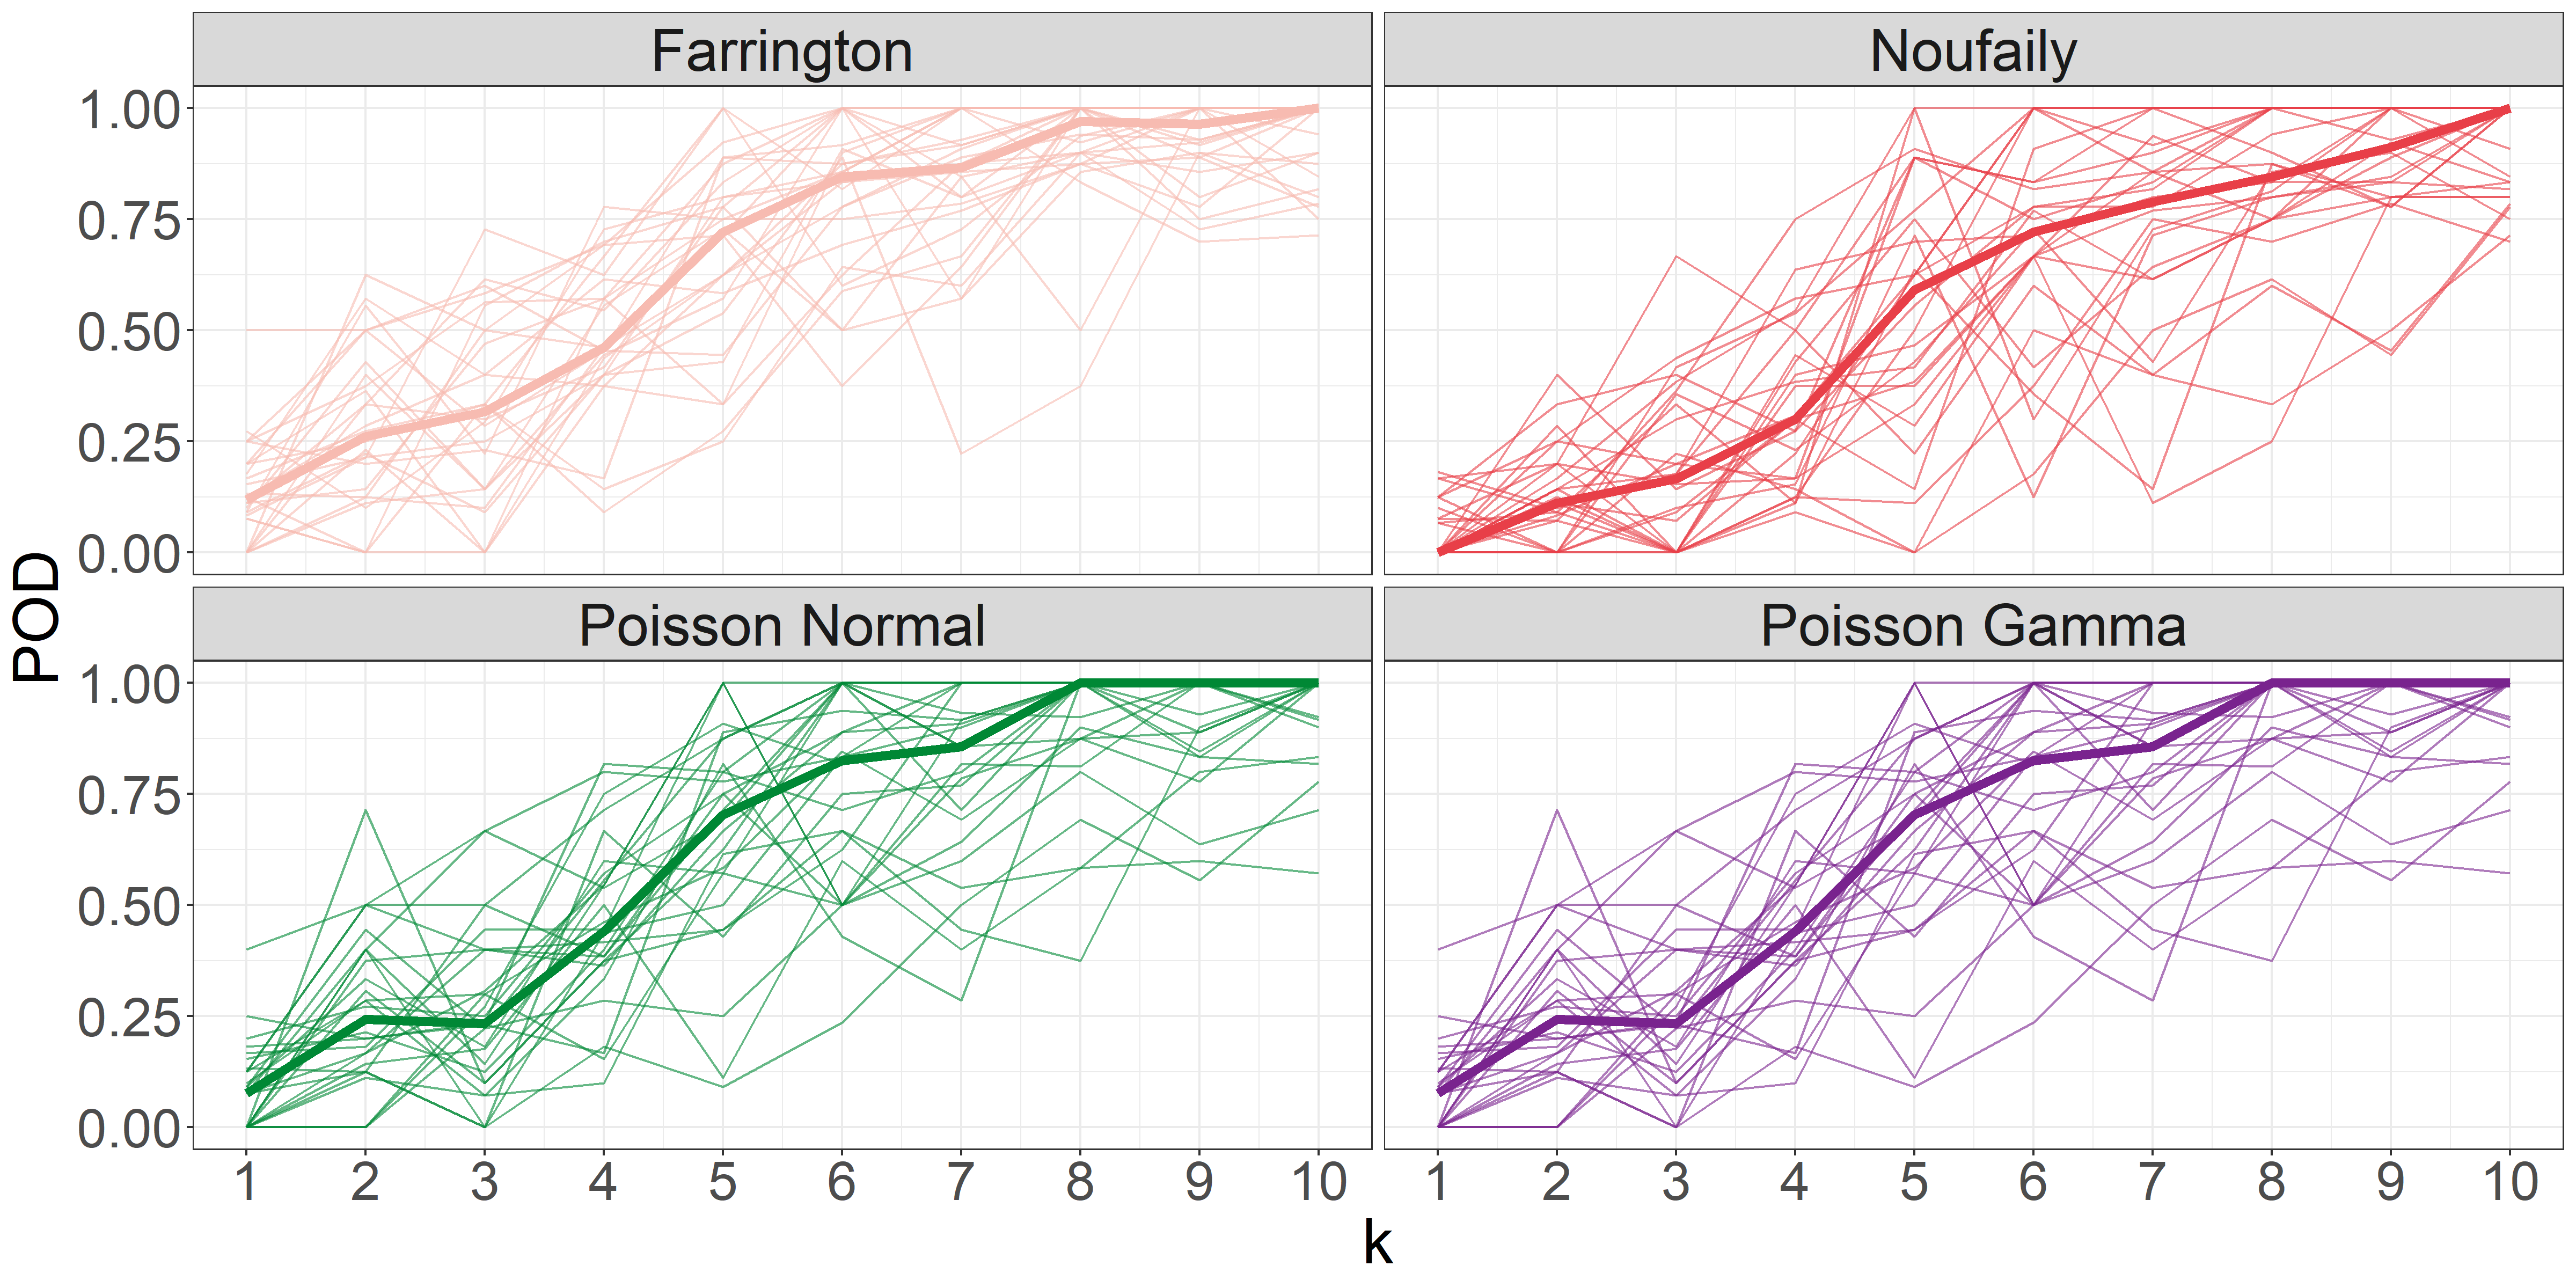
\includegraphics[width=1\linewidth]{../figures/PropDetect}

\normalsize
\end{frame}

\hypertarget{profile-of-pod-vs-fpr}{%
\subsection{Profile of POD vs FPR}\label{profile-of-pod-vs-fpr}}

\begin{frame}{Profile of POD vs FPR}
\tiny

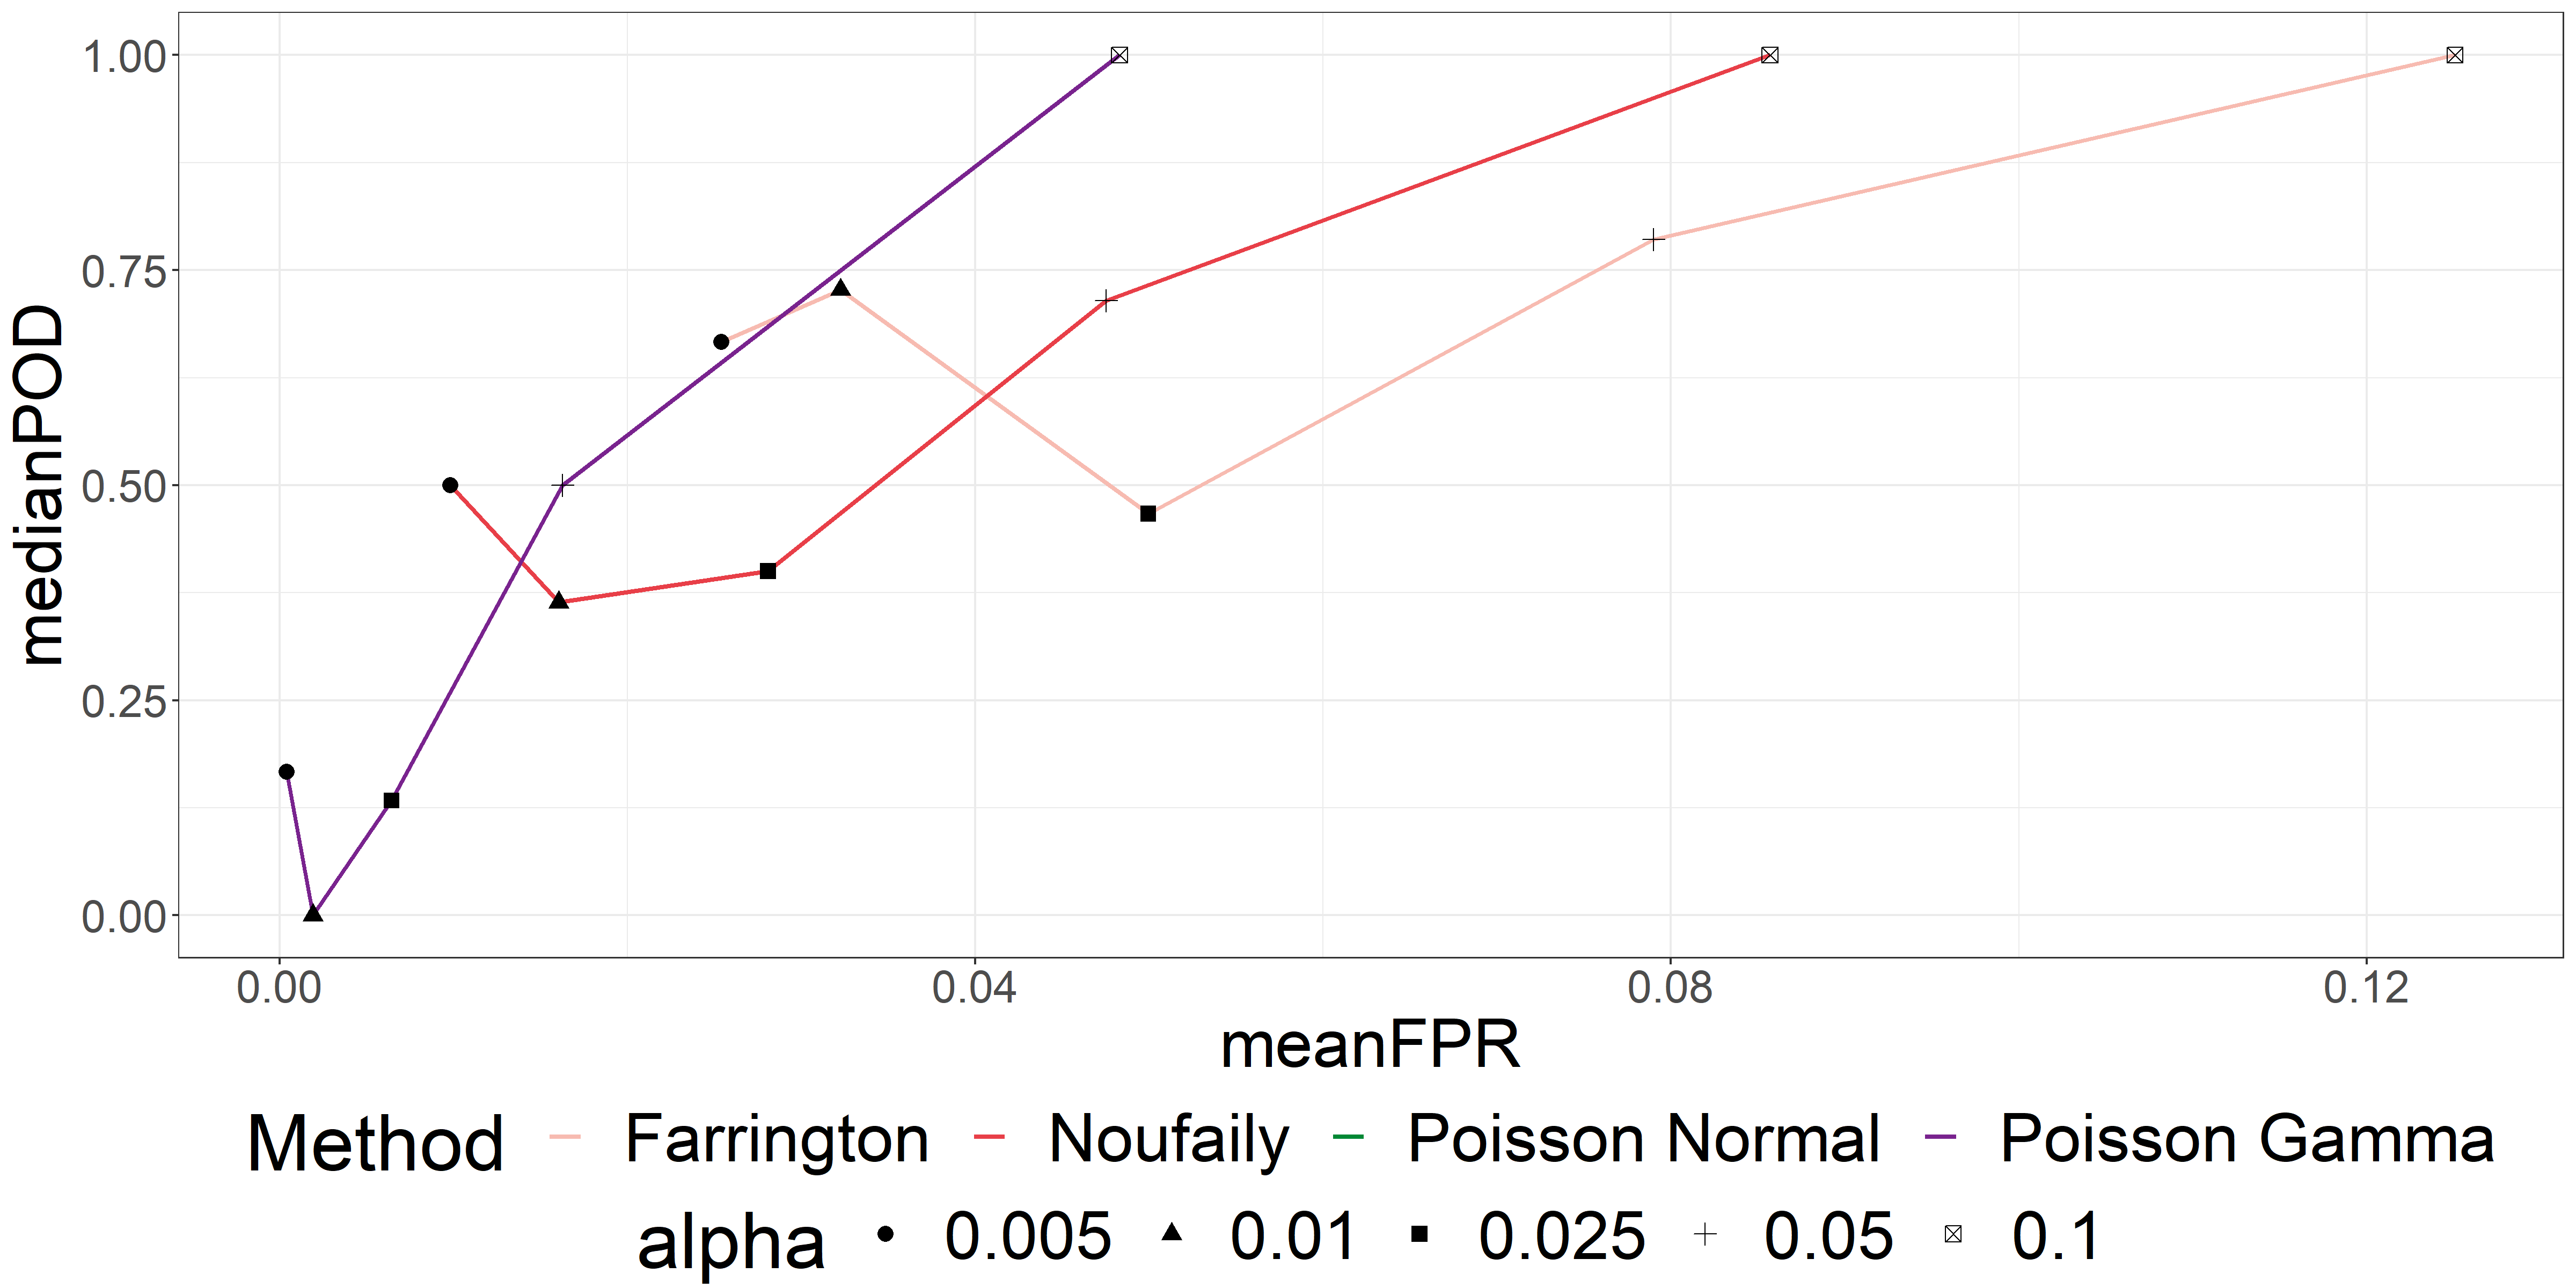
\includegraphics[width=1\linewidth]{../figures/profilePODxFPR_shape}

\normalsize
\end{frame}

\hypertarget{profile-of-pod-vs-fpr-for-different-outbreak-sizes}{%
\subsection{Profile of POD vs FPR for different outbreak
sizes}\label{profile-of-pod-vs-fpr-for-different-outbreak-sizes}}

\begin{frame}{Profile of POD vs FPR for different outbreak sizes}
\tiny

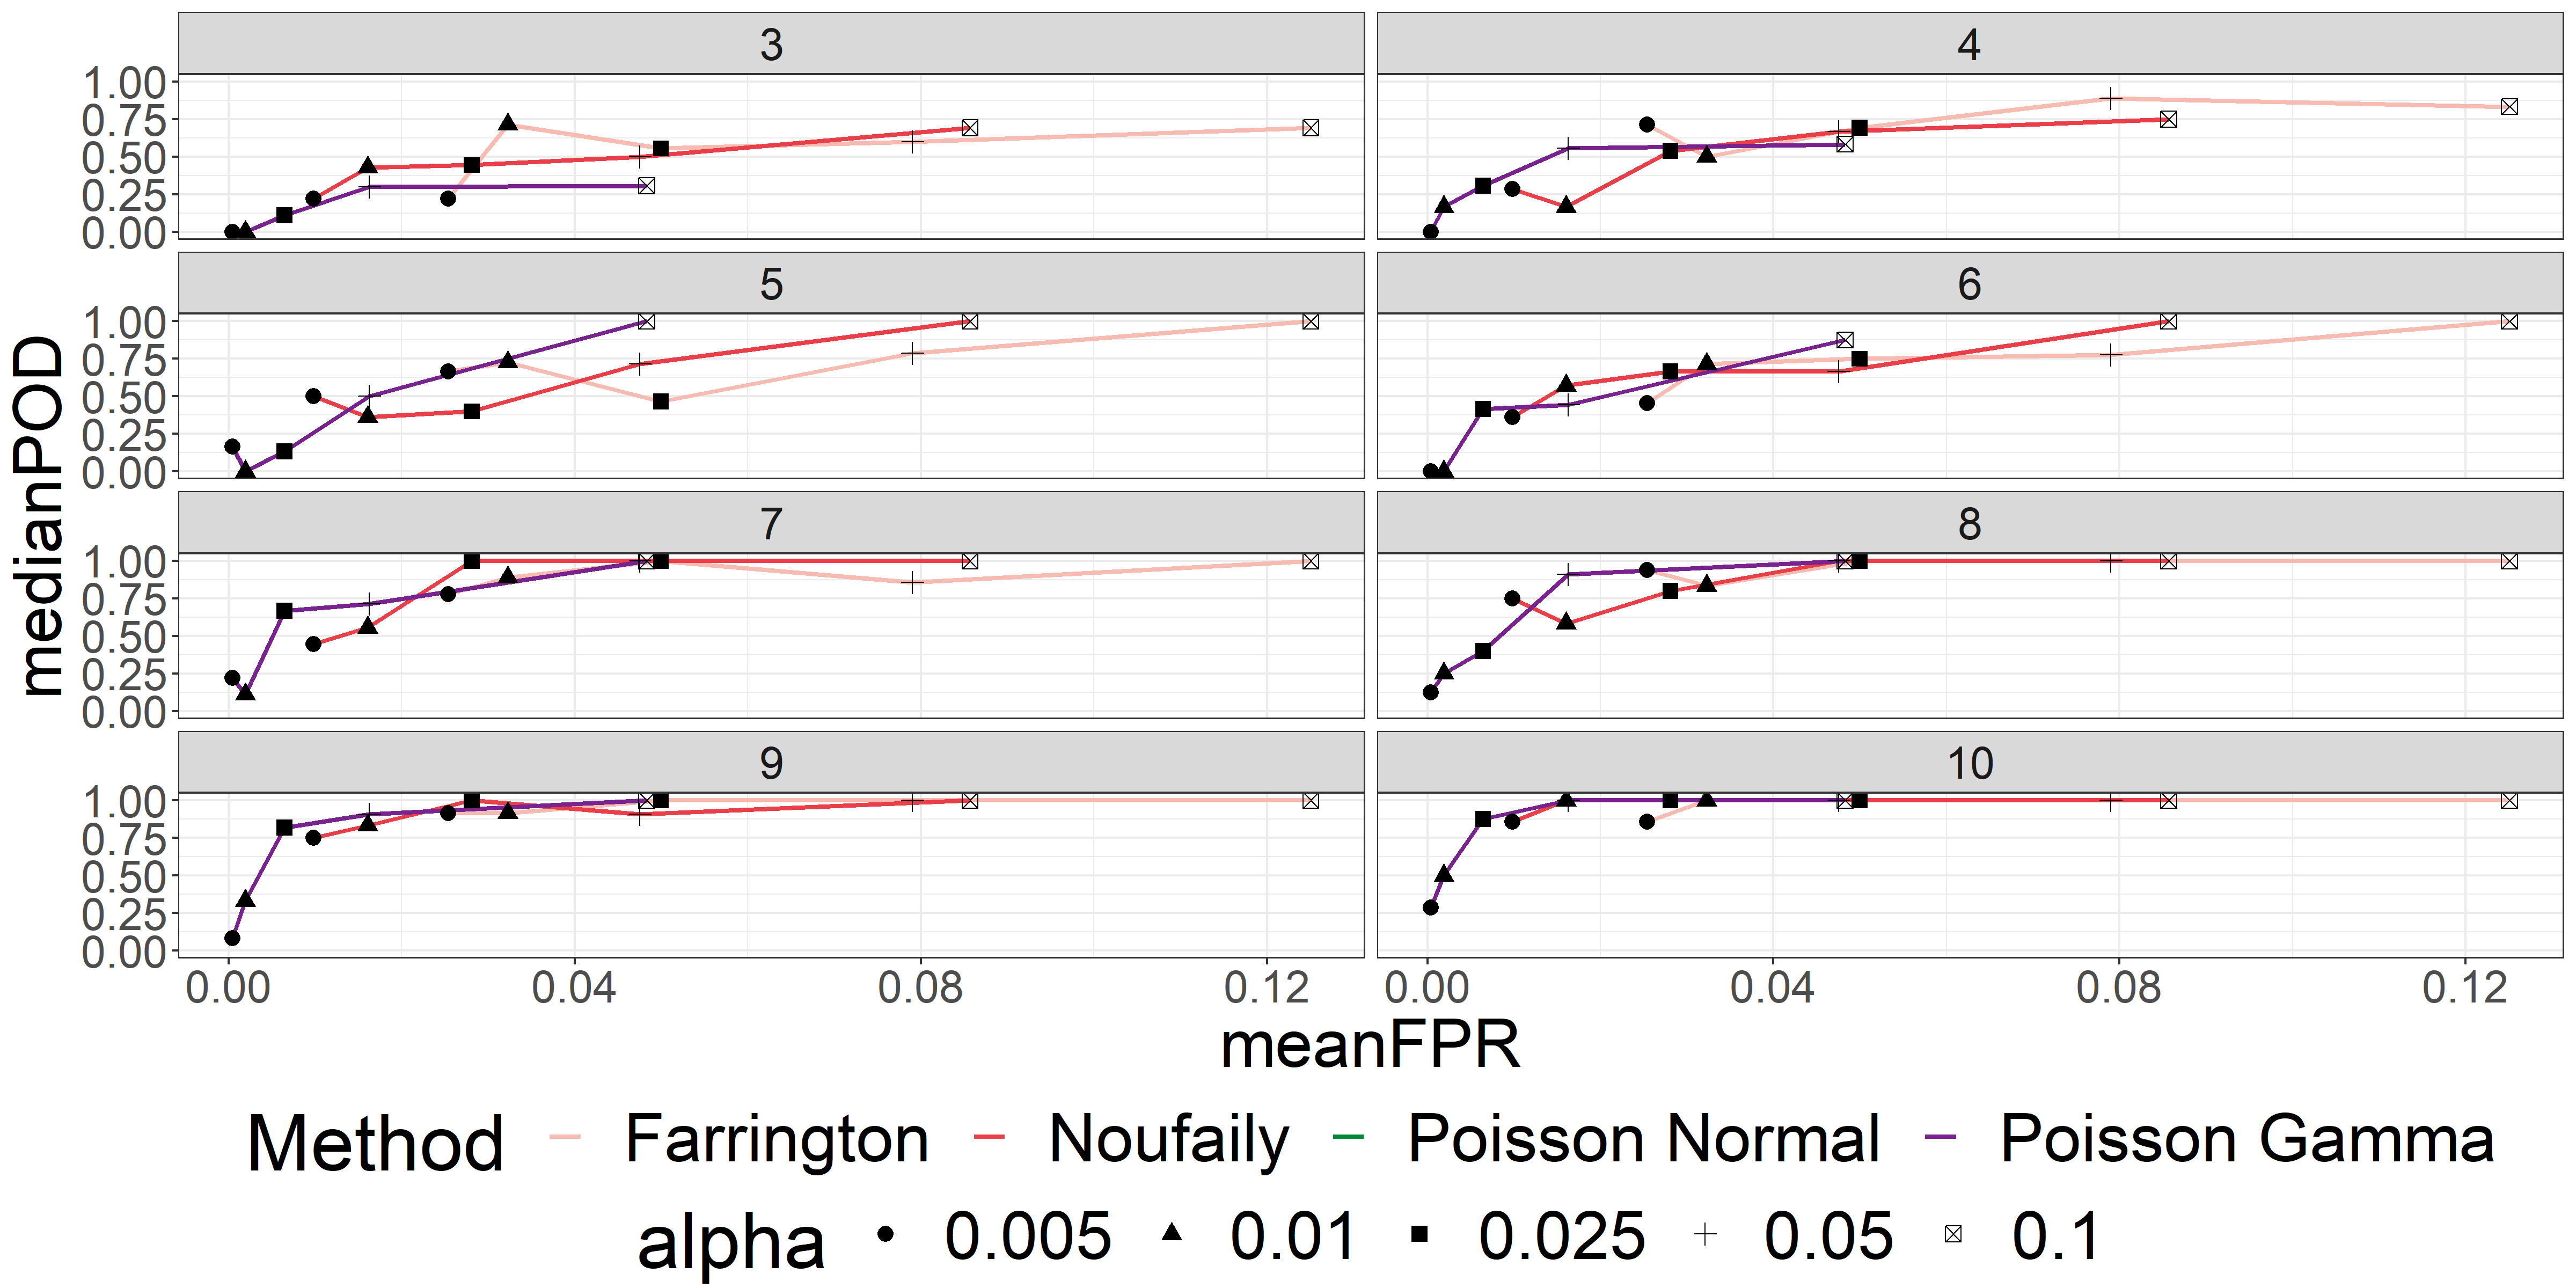
\includegraphics[width=1\linewidth]{../figures/profilePODxFPR_facet}

\normalsize
\end{frame}

\hypertarget{summary}{%
\section{Summary}\label{summary}}

\begin{frame}{Summary}
\begin{itemize}
  \item Easy incorporation of \textbf{covariates}
  \item Estimates are \textbf{consistent} across the two modeling frameworks
  \item Positively \textbf{identified outbreaks} coinciding with well-documented outbreaks
  \item Effectively \textbf{control the number of "false alarms"}
  \item Great potential in utilizing \textbf{MiBa-based surveillance}
\end{itemize}
\end{frame}

\hypertarget{references}{%
\section{References}\label{references}}

\begin{frame}{References}
\printbibliography[heading=none]
\end{frame}

\hypertarget{hierarchical-poisson-gamma-model}{%
\section{Hierarchical Poisson Gamma
model}\label{hierarchical-poisson-gamma-model}}

\hypertarget{probability-function-for-y}{%
\subsection{\texorpdfstring{Probability function for
\(Y\)}{Probability function for Y}}\label{probability-function-for-y}}

\begin{frame}{Probability function for \(Y\)}
\begin{equation} \label{eq:pdfMix}
  \begin{aligned}
    P[Y=y]&=g_{Y}(y;\boldsymbol \beta, \phi) \\
    &=\frac{\lambda^{y}}{y!\Gamma(1/\phi)\phi^{1/\phi}}\frac{\phi^{y+1/\phi}\Gamma(y+1/\phi)}{(\lambda \phi + 1)^{y+1/\phi}} \\
    &=\frac{\Gamma(y+1/\phi)}{\Gamma(1/\phi)y!}\frac{1}{(\lambda\phi+1)^{1/\phi}}\bigg(\frac{\lambda\phi}{\lambda\phi+1}\bigg)^{y} \\
    &=\begin{pmatrix} y+1/\phi-1 \\ y \end{pmatrix} \frac{1}{(\lambda\phi+1)^{1/\phi}}\bigg(\frac{\lambda\phi}{\lambda\phi+1}\bigg)^{y} \ , \quad \mathrm{for} \ y = 0, 1, 2, \dots
  \end{aligned}
\end{equation}

where the following convention is used

\begin{equation}
  \begin{pmatrix} z\\y \end{pmatrix} = \frac{\Gamma(z+1)}{\Gamma(z+1-y)y!}
\end{equation}

The marginal distribution of \(Y\) is a negative binomial distribution,
\(Y\sim \NB\big(1/\phi,1/(\lambda \phi+1)\big)\)
\end{frame}

\hypertarget{proof}{%
\subsection{Proof}\label{proof}}

\begin{frame}{Proof}
The probability function for the conditional distribution of \(Y\) for
given \(u\)

\begin{equation}\label{eq:pdfPois}
  f_{Y|u}(y;u,\boldsymbol{\beta})=\frac{(\lambda u)^{y}}{y!}\exp(-\lambda u)
\end{equation}

and the probability density function for the distribution of \(u\) is

\begin{equation} \label{eq:pdfGamma}
  f_{u}(u;\phi)=\frac{1}{\phi \Gamma(1/\phi)} \bigg(\frac{u}{\phi}\bigg)^{1/\phi-1} \exp (-u/\phi)
\end{equation}
\end{frame}

\begin{frame}{Proof}
\protect\hypertarget{proof-1}{}
Given \eqref{eq:pdfPois} and \eqref{eq:pdfGamma}, the probability
function for the marginal distribution of \(Y\) is determined from

\begin{equation} \label{eq:marMix}
  \begin{aligned}
    g_{Y}(y;\beta,\phi)&=\int_{u=0}^\infty f_{Y|u}(y;u,\beta) f_{u}(u;\phi) \,du \\
    &=\int_{u=0}^\infty \frac{(\lambda u)^y}{y!} \exp (-\lambda u) \frac{1}{\phi \Gamma(1/\phi)} \bigg(\frac{u}{\phi}\bigg)^{1/\phi-1} \exp (-u /\phi) \,du\\
    &=\frac{\lambda^{y}}{y!\Gamma(1/\phi)\phi^{1/\phi}} \int_{u=0}^\infty u^{y+1/\phi-1} \exp \big(-u(\lambda \phi+1)/\phi\big) \,du
  \end{aligned}
\end{equation}
\end{frame}

\begin{frame}{Proof}
\protect\hypertarget{proof-2}{}
In \eqref{eq:marMix} it is noted that the integrand is the \emph{kernel}
in the probability density function for a Gamma distribution,
\(\G\big(y+1/\phi,\phi/(\lambda \phi+1)\big)\). As the integral of the
density shall equal one, we find by adjusting the norming constant that

\begin{equation}
  \int_{u=0}^\infty  u^{ y+ 1/\phi-1} \exp \Big(- u/\big(\phi/( \lambda \phi+1)\big)\Big) \,du = \frac{\phi^{ y+ 1/\phi}\Gamma( y+\boldsymbol 1/\phi)}{( \lambda \phi + 1)^{y+1/\phi}}
\end{equation}

and then \eqref{eq:pdfMix} follows
\end{frame}


\end{document}
